\documentclass[a4paper,11pt,twoside]{article}
\usepackage[T1]{fontenc}
\usepackage{ae}
\usepackage[latin1]{inputenc}
% \usepackage[finnish]{babel}
\usepackage{newcent}
\usepackage{graphicx}
\usepackage{booktabs}
\usepackage{url}
\usepackage{moreverb}
\usepackage{lscape}
\usepackage{longtable}
\frenchspacing
 
% \oddsidemargin 0cm
% \evensidemargin 0cm
% \textheight = 20cm
% \textwidth = 15cm

\pagestyle{plain}

\newcommand{\texlipse}{\TeX lipse}


\begin{document}

% \renewcommand{\thepage}{\roman{page}}
\pagenumbering{roman}

\begin{titlepage}
\strut
\begin{minipage}{\textwidth}
\LARGE {\bf T-76.115 Technical Specification}\\
\LARGE {\bf \TeX lipse project}\\
\LARGE {\bf Group TeXlapse}
\end{minipage}

\addvspace{2cm}
\begin{minipage}{\textwidth}
\large{ID: TEXLIPSE-TECH-1}\\
\large{Version: 1.8}\\
\large{Modified: \today}\\
\\
\large{Author:\\ Oskar Ojala (omojala@cc.hut.fi)}
\end{minipage}

\end{titlepage}

%\pagestyle{plain}

\clearpage


\begin{table}[!htpb]
\begin{center}
\caption{Version history}
\begin{tabular}{lllp{60mm}}
Version & Date & Editor & Change \\
\midrule
0.1 & 14.11.2004 & Oskar & Basic structure\\
0.2 & 22.11.2004 & Kimmo & File output and building\\
0.3 & 22.11.2004 & Esa & Templates and preview\\ 
0.4 & 25.11.2004 & Taavi & Viewing the outline, Basic outline navigation\\
0.5 & 25.11.2004 & Oskar & Some architecture and technical descriptions added\\
0.6 & 25.11.2004 & Esa & Added template syntax\\
0.7 & 26.11.2004 & Esa & Modified template sections and appendix\\
0.8 & 28.11.2004 & Oskar & Made corrections based on inspection, added some technical details\\
0.9 & 29.11.2004 & Oskar & Added more technical detail in tasks and did some corrections\\
1.0 & 29.11.2004 & Kimmo & Added some more explanations about the builder\\
1.1 &   4.1.2005 & Kimmo & Updated the builder diagram and explanation of it\\
1.2 &  29.1.2005 & Oskar & Added folding support and made some adjustments\\
1.3 &   1.2.2005 & Kimmo & Added previewer explanation and diagram\\
1.4 &   7.2.2005 & Oskar & Updated most of the document, made new architectural diagrams\\
1.5 &  11.3.2005 & Oskar & Updated the parsing section\\
1.6 &  12.3.2005 & Oskar & Read and updated nearly entire document, rewrote template part\\
1.7 &  13.3.2005 & Taavi & Updated the outline related implementation task stuff\\
1.8 &  13.3.2005 & Oskar & Proofread and corrected outline description\\
\end{tabular}
\end{center}
\end{table}


\clearpage
\tableofcontents
\clearpage

\pagenumbering{arabic}

\parindent 0em
\parskip 10pt

\section{Purpose and scope of the document}

The purpose of this document is to define the technical specification and 
architecture of the \texlipse\ system. This is intended to complement the 
\texlipse\ requirements documentation. Thus, this document focuses primarily on 
specifying how features are to be implemented and why they are implemented in 
the specified way. Secondarily, this document focuses on defining feature 
behavior more specifically than done in the requirements document when that is 
necessary for implementing the requirement.

\subsection{Prerequisites}

The intended audience of this document is people interested in the architecture 
and implementation of \texlipse\ and have some degree of programming background.

To fully comprehend the contents of this document, knowledge of the Eclipse 
plugin architecture, the \TeX\ typesetting system and of compiler techniques is 
required. These topics are so broad that it's impossible to summarize them 
here, however compiler and \TeX\ -resources are referred to when appropriate 
and Eclipse documentation can be found at the Eclipse www-site 
\mbox{(\url{http://www.eclipse.org})}.

This document can be read with only knowledge of the requirements (see the 
document TEXLIPSE-REQ-1) and Eclipse with the help of the domain concept 
descriptions, but in some places there are technical descriptions that require 
more in-depth knowledge, and these may thus be skipped if the reader merely 
wants an overview.

\subsection{Document structure}

The rest of this document is organized as follows: Section~\ref{sect:concepts} 
introduces the key concept in the architecture and technical design of 
\texlipse. Section~\ref{sect:overview} makes a fairly detailed architectural 
overview of the key concepts of \texlipse\ and the software structure chosen. 
Section~\ref{sect:technover} expands on the architecture description and 
explains in more detail how the different parts are implemented and, most 
importantly, how they work together. Section~\ref{sect:techntasks} explains 
more detailed implementation-level issues and techniques used per 
implementation tasks (the tasks correspond fairly well to the functional 
requirements of \texlipse).


\section{Main domain concepts}
\label{sect:concepts}

Main domain concepts:

\begin{description}

\item[AST] Abstract Syntax Tree, a tree representation of the parsed
  stream. In contrast to CST, only selected tokens are represented and
  superfluous tokens (such as expression terminators and parentheses)
  are ignored in the tree.

\item[Bib\TeX] A bibliography citation inclusion system for \LaTeX ,
  developed by Oren Patashnik. Uses a bibliography file and a style file
  to make a bibliography list to the \LaTeX\ document and to include
  only the cited bibliographies. See~\cite{Lamport:LDP85} 
  and~\cite{Patashnik:Bib-TUG-03-1}.

\item[CST] Concrete Syntax Tree, a tree representation of the parsed
  stream as recognized by the parser. Each token have their appropriate
  place in the tree dictated by the grammar.

\item[DFA] Deterministic Finite Automaton, an automaton that has 
  deterministic state transitions, useful for representing regular 
  expressions in computer-executable form, thus used for building
  lexers.

\item[EBNF] Extended Backus Naur Form, the common way of describing
  context-free grammars.

\item[Eclipse IDE] A free Integrated Development Environment sponsored
  by IBM. Intended originally for Java development, but currently
  emphasizes plugins for adding functionality beyond the original
  requirements.
  
\item[Eclipse plugin] A piece of Java software that integrates with
  the Eclipse plugin architecture and provides some additional feature
  for the Eclipse environment.

\item[Eclipse plugin framework] The Eclipse platform offers a rich
  framework for plugins, complete with interfaces and classes for
  implementing many common functions more easily.

\item[Editor] In Eclipse the editor view, or editor for short (as it's
  used throughout this document) is a view where the documents can be
  edited as in a normal text editor. The editor can be extended with 
  many kinds of functionality, such as syntax highlighting.

\item[GUI widget] A component in the GUI (Graphical User Interface);
  can be a button, a window, a checkbox, a menu, etc.

\item[LALR] Look-ahead LR, a LR parsing method that is more powerful
  than the SLR method, but easier than the LR-method without
  sacrificing too much in recognized languages. See LR.

\item[\LaTeX] A popular typesetting language, based on \TeX. Is
  written as a plain text file with a series of commands. 
  See~\cite{Lamport:LDP85}.

\item[Lexer] A program for reading a stream and recognizing predefined
  tokens in the stream, then returning found tokens or an error if the
  stream doesn't correspond to the specified format.
  
\item[LL] Left to right, leftmost derivation parsing, an easy to
  understand top-down family of parsing methods. Refer
  to~\cite{Aho:CPT86} for details.

\item[LR] Left to right, rightmost derivation parsing, a family of
  bottom-up parsing methods. Refer to~\cite{Aho:CPT86} and see
  also~\cite{Knuth:j-IC-8-6-607}.

\item[MVC] Model-View-Controller, a design pattern where the date is held
  in a model, the data is presented through views and the mapping of data
  to views and vice versa is done by the controller.

\item[Outline] In Eclipse the outline view, or outline for short (as it's
  used throughout this document) is a view where the currently edited 
  document's (the document that is currently shown in the editor) structure is 
  shown. For examples, in the case of a Java class it would include all the 
  fields and methods, and in the case of a \LaTeX -document it would include the
  sections.

\item[Parser] A program for checking that tokens match a 
  predefined grammar, ie\. to check that the given stream is of the
  right form.
  
\item[Parser generator] A software for automatically generating a
  lexer and a parser from a given grammar specification.

\item[Singleton] A design pattern where the singleton class only has
  one existing object instance at any time, which is then shared among
  other runtime objects.

\item[\TeX] A powerful typesetting system that permits the user to typeset
  documents in professional quality by using a flexible command
  language. See~\cite{Knuth:texbook84} for a description of the language,
  \cite{Knuth:texprogram86} for a description of how \TeX\ works.

\item[View] In Eclipse, there are several views: the editor view, 
  the outline view, the problems view, etc. These are different views on
  the document or project being edited and appear visually as separate 
  areas in the Eclipse GUI.

\item[Visitor] A design pattern where an object, which is the visitor,
  visits another object, thereby performing a number of operations on
  the visited object. The visitor implements a certain interface, so
  that it can be applied to the visited object. In \texlipse, visitors 
  are used for trees, so that the visited object calls a method 
  defined in the visitor interface when a node corresponding to the 
  method is visited in the tree. See~\cite{Gagnon:mth-98} for a more
  thorough explanation.

\end{description}


\section{System overview}
\label{sect:overview}

\texlipse\ is a plugin for the Eclipse IDE. It provides a \LaTeX\ editor for 
editing and building \LaTeX\ documents.

Briefly, it provides automatic completion of references, syntax highlighting, user 
defined templates, automatic building, previewing, error reporting and an 
outline view. It does not re-implement \LaTeX, rather, it is intended to serve 
as a powerful editing tool for \LaTeX\ documents. It does not implement WYSIWYG 
editing of the document, as it is intended to be a power user tool to speed up 
editing of \LaTeX\ source. Refer to the \texlipse\ requirements document 
(document ID TEXLIPSE-REQ-1) for more information about the intended use and 
features of the system.


\section{Architectural overview}
\label{sect:archover}

\subsection{About plugins}

The Eclipse plugin architecture places many constraints on the structure of the 
plugin. Essentially, the Eclipse platform provides much infrastructure for 
building an editing environment, e.g.\ the plugin developer does not need to 
program GUI widgets and basic editing functions such as copy and paste by 
himself. On the other hand, the Eclipse platform and the ready-made 
infrastructure places certain constraints on the architecture, e.g.\ how 
documents are handled. In general, the wins provided by the (extensive) 
ready-made functionality far outweigh the disadvantages.

\begin{figure}[!htp]
\begin{center}
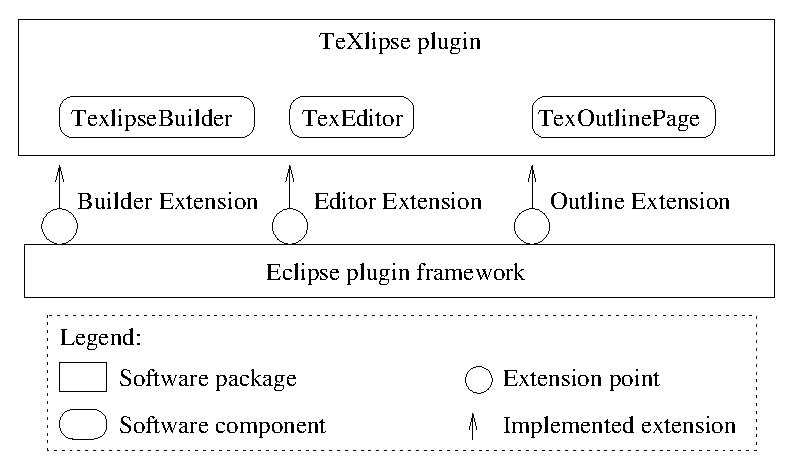
\includegraphics[width=9cm]{images/plugin}
\caption{The plugin structure: \texlipse\ extends Eclipse on certain extension points}
\label{fig:plugin}
\end{center}
\end{figure}

The plugin is not a standalone piece of software; it integrates tightly with 
Eclipse. Figure~\ref{fig:plugin} depicts this and also shows three central 
components of \texlipse: the editor, representing the editor view, the outline, 
representing the outline view and the builder, which handles interfacing to 
external programs (e.g.\ \LaTeX) that are needed to build the document. The 
editor and outline directly represent the Eclipse views of the same names and 
thus build on the Eclipse plugin framework. The builder is the core component 
in a set of components handling interfacing to external programs that handle 
building and previewing \LaTeX\ documents.


\subsection{External interfaces}

To see how the \texlipse\ plugin fits in in the user's programming
environment, see Figure~\ref{fig:ext}, which presents the external
interfaces of the plugin and the control flow. In order to work, the
plugin requires (besides Eclipse) tools for actually compiling the
created documents into vector representations, i.e.\ postscript, dvi,
and/or pdf. Thus, a \LaTeX\ distribution is required to be installed
separately, which \texlipse\ then calls to parse the document.
For implementation details, see Section~\ref{sect:t3.1}.

For previewing the created document, an external previewer is called.
The \texlipse\ plugin permits the previewer to send messages back to
the plugin, enabling bidirectional communication which makes
synchronizing the Eclipse document view and the previewer view
possible. For implementation details, see Section~\ref{sect:t3.4}.

\begin{figure}[!htp]
\begin{center}
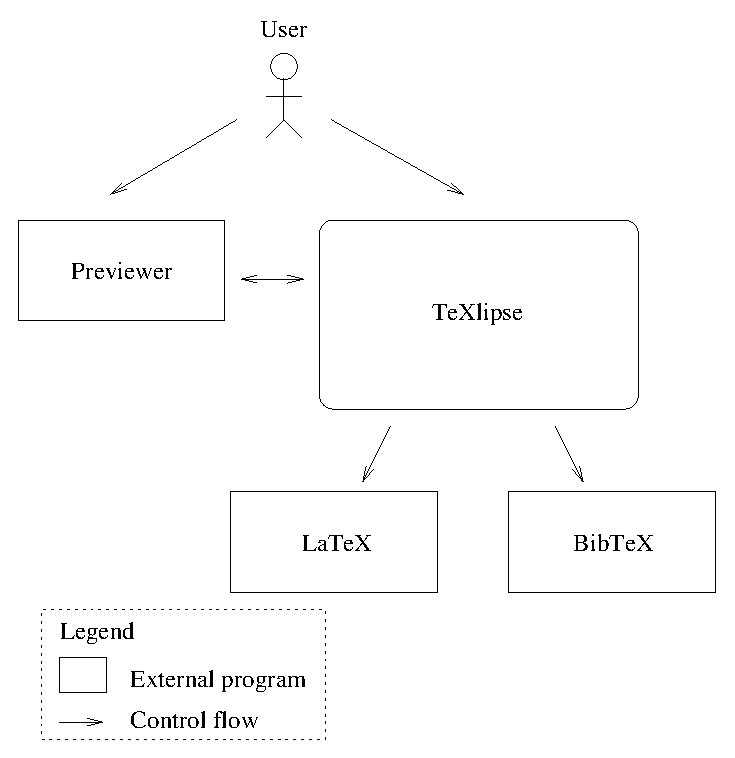
\includegraphics[width=10cm]{images/external}
\caption{External interfaces with control flows depicted}
\label{fig:ext}
\end{center}
\end{figure} 

Due to the fact that \texlipse\ is designed to run on three different
operating systems, all having somewhat different facilities, preferred
distributions of \LaTeX\ and different previewers, the external
interfaces to programs must be able to handle all of these fairly
invisibly to the user (the user is naturally required to set up the
system, but setting up \texlipse\ shouldn't differ too much on different
platforms).

Beside program interfaces such as calling \LaTeX\ or a previewer,
Figure~\ref{fig:ext} includes the user. The user mostly works with the
editor, which provides the direct editing view of the document
source. The user also works with the document outline, the file system
browser (provided automatically by Eclipse) and the problems view in
the Eclipse GUI. The user can activate the builder and the
previewer. Thus, the user has the interface of different views (the editor,
document outline, the problems log and the console) to the document, but can
also control the activation of building the document and previewing it from 
\texlipse.


\subsection{Document model}
\label{sect:archdm}

The core concepts in \texlipse\ are focused around the editor view and its 
functions. \texlipse\ provides a \LaTeX -editor and other useful views on the 
document being edited, the central one of them being the document outline view. 
The outline view shows a document outline as described in requirement R2.1 
(requirement document ID TEXLIPSE-REQ-1). In order to implement some editor and 
outline functions, parsers for Bib\TeX\ and \LaTeX\ are implemented (these are 
described in more detail in Section~\ref{sect:techparse}).

In order to facilitate the necessary communication between the outline, the 
editor and the document parser(s), the MVC (Model-View-Controller) pattern is 
applied in an adapted form. In this pattern, we have the model representing the 
data, the view representing a view on the data (typically a GUI) and the 
controller representing the logic for mapping different data to different 
views. This pattern is particularly useful in GUIs, since the order of user 
interaction cannot be known in advance, enabling the data to be edited from 
different views and it provides an order of abstraction between the GUI and the 
data model.

In an Eclipse plugin one doesn't need to implement the GUI from scratch --- in 
fact, the GUI comes largely ready from the existing plugin infrastructure, so 
the ``view'' part is a quite thin. Also, the Eclipse plugin structure places 
some constraints on the document model and object hierarchy, so the MVC pattern 
is adapted to our needs. Figure~\ref{fig:emop} shows the coupling of the 
central editing views; Model keeps abstract representations of the document 
(autocomplete data and outline data), asking the parsers to return updated 
versions of the data structures when the data itself is updated. The editor 
essentially provides information on editing updates and fetches new data
structures, as does the outline.

\begin{figure}[!htp]
\begin{center}
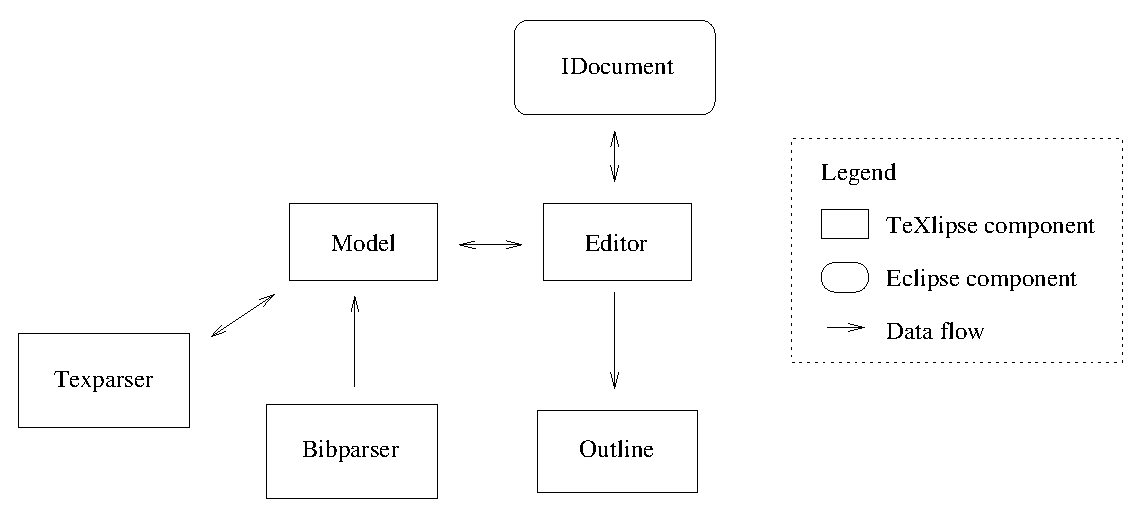
\includegraphics[width=10cm]{images/emop}
\caption{Editor-Model-Outline-Parser MVC-style coupling}
\label{fig:emop}
\end{center}
\end{figure} 

It's worth to note that in Figure~\ref{fig:emop}, \texttt{IDocument} is an 
Eclipse class, which contains the document being edited. The plugin 
architecture automatically provides for this, but \texttt{IDocument} is not 
alone sufficient in holding all the data required (e.g.\ the outline structure), 
so we augment it with the model that contains somewhat more abstract 
representations of the document, in contrast to the concrete representation of 
\texttt{IDocument}. Thus, \texttt{IDocument} holds the model of the concrete 
file-based document, while our model holds the model for \LaTeX -specific 
abstractions.

The reader might ask why use the MVC paradigm in such a way that the controller 
is distributed into several classes and there are essentially two models? 
First, the Eclipse plugin platform provides the basic way of operation for the 
editor and outline, as well as the \texttt{IDocument}, so the developer doesn't 
have too much leeway. Second, our model can be thought of as a controller, 
except that there are circumstances where it's more efficient and simple for 
the editor and the outline to go directly to \texttt{IDocument}. Third, this 
behavior is much better than a casual glance would suggest, since 
\texttt{IDocument}-class changes only if Eclipse changes and such a major 
change that would require a major rewrite of \texlipse\ would require a major 
rewrite of a significant number of plugins, making the change unlikely. Fourth, 
the pattern described already provides a good degree of abstraction; the 
parsers may be changed at will, without having any effect on other components 
than model, since the data interfaces to it are standardized. In practice, the
abstract data structures contained in Model are necessary for many functions of
\texlipse, so they must be stored in some way. This mechanism employs the
bridge-pattern for abstracting the parser interface from the parser's
implementation and a facade-pattern for hiding the parsing stages behind the
model (see~\cite{GHJV:despatterns95} for more information).

While developing \texlipse\ 1.0, this means of abstraction proved to work very
well, as the the technically demanding parsers and the model infrastructure
could both be developed independently from the rest of the system, making
development both less risky in terms of new bugs introduced and easier to
parallelize since other developers didn't need to wait for the parsers or model
to be refined.


\subsection{System architecture}

Figure~\ref{fig:arch} presents the \texlipse\ architecture. As can be expected, 
the editor is a central piece in the plugin. In Figure~\ref{fig:arch}, the 
Eclipse plugin infrastructure is not shown for reasons of clarity. Thus, the 
builder appears not to be connected to anything else than the editor, even 
though it most certainly is --- the Eclipse plugin architecture handles calling 
it. This situation is depicted in Figure~\ref{fig:plugin}; the central parts of 
\texlipse's interface with the Eclipse plugin architecture, which provides the 
connecting framework.

\begin{figure}[!htp]
\begin{center}
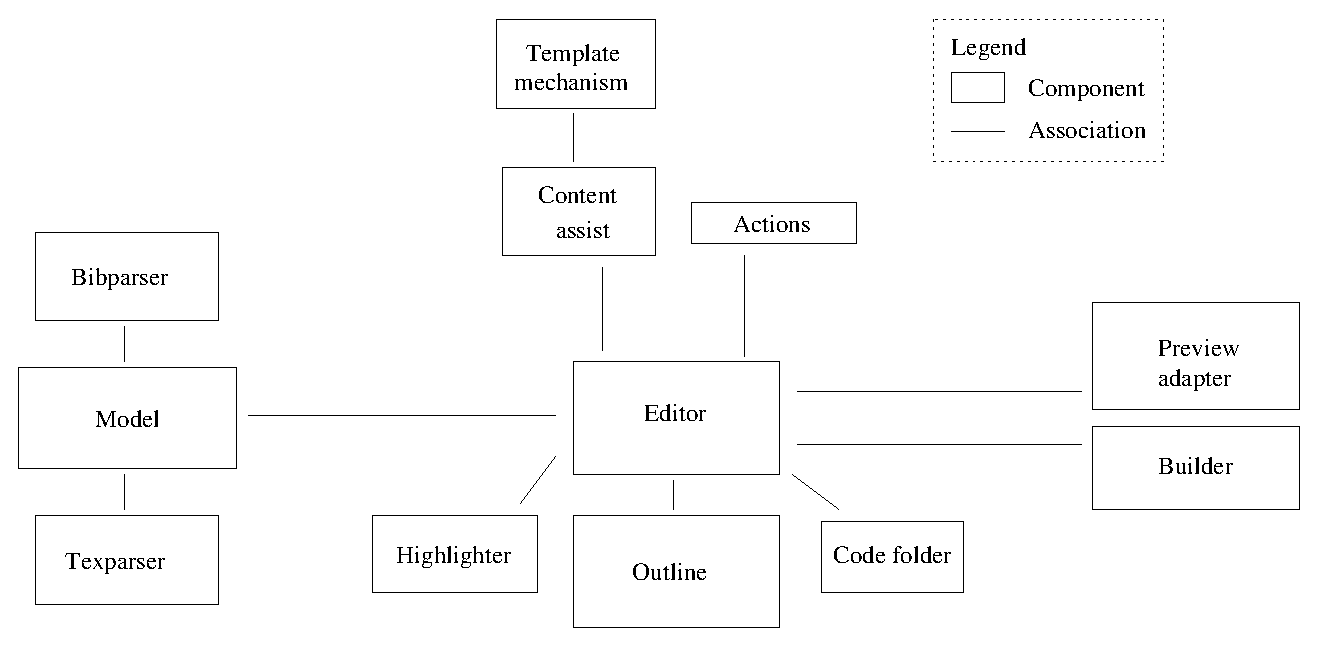
\includegraphics[width=11cm]{images/architecture}
\caption{\texlipse\ architecture shown as a component view}
\label{fig:arch}
\end{center}
\end{figure} 

The architecture, as shown in Figure~\ref{fig:arch}, introduces some new parts 
--- the template mechanism, the actions, content assist, the highlighter and 
the code folder. The actions are the simplest --- they simply contain editor 
actions for error messages and menu options (e.g.\ indenting or commenting a 
selected region of text is triggered from the actions). The template mechanism 
is also closely associated with the editor and provides the mechanism for 
retrieving templates (both pre-made and user defined) as well as enabling the 
use of templates while editing. There are two kinds of templates: document 
templates and editing templates. The former can be applied to the entire 
document/project when starting a new project. The latter can be used via typed 
abbreviations during editing and they insert a template into the document being 
edited. Due to this difference, both use entirely separate mechanisms. The 
actual template completions, along with reference and command completions are 
handled by the content assistant --framework.

The code folder handles folding away parts of the \LaTeX -source from
the editing view and the highlighter is a major component handling the
syntax highlighting in the editor.

The external interfaces were already discussed and they consist of two
major parts: the previewing facilities and the building facilities
The preview adapter interfaces the document preview with the
editor so that both views can be synchronized when a previewer that
supports this functionality is used. The builder handles the building
of the document and thus interfacing to the \LaTeX\ and Bib\TeX
-programs installed. It calls them and they in turn produce the
document in the desired format.



\section{Technical overview}
\label{sect:technover}

Based on the architecture described in Section~\ref{sect:archover} we
have developed a technical design. The technical design encompasses
the package and class structure of \texlipse, as well as the
interaction between the different components.


\subsection{Packages}

Table~\ref{tbl:pkg} summarizes the package structure of the plugin and
briefly describes what each package does. Note that the base package
is fi.hut.soberit.texlipse, which has been omitted from the table for
brewity.

\begin{table}[!htpb]
\begin{center}
\begin{tabular}{lp{10cm}}
package & function \\
\midrule
plugin & Plugin base functionality\\
actions & Editor actions (e.g.\ code commenting)\\
bibeditor & Bib\TeX\ editor functionality\\
bibparser & Bib\TeX\ parser\\
builder & Builder functionality\\
editor & Editor and associated functionality\\
editor.scanner & Syntax highlighting; partition scanners and rules\\
model & Abstract document model\\
outline & Outline view\\
parenmatcher & Paren matching functionality\\
properties & Project property pages\\
tableview & Table editor view\\
templates & Template functionality\\
texparser & \LaTeX\ parser\\
viewer & Previewer functionality\\
wizards & Wizards (e.g.\ project creation)\\
%\hline
\end{tabular}
\end{center}
\caption{Package structure; the base package is fi.hut.soberit.texlipse}
\label{tbl:pkg}
\end{table}

It must be noted that Table~\ref{tbl:pkg} omits automatically generated parser 
packages (lexer, parser, node and analysis) under both parser packages --- most 
of the automatically generated code is not meant to be human-readable and is 
abstracted neatly through the classes in the base parser packages.


\subsection{Document model}

The architecture behind the \texlipse\ document model was described in 
Section~\ref{sect:archdm}. Here we proceed to define how we process the 
document and what classes are involved in some of the basic document-handling 
functions.


\subsubsection{Parsing}
\label{sect:techparse}

For simplicity, the mechanism of parsing a Bib\TeX\ document is presented here, 
rather than the \LaTeX\ parser. The basic idea is the same, but parsing 
Bib\TeX\ is simpler and the internal structure is more elegant (despite the 
fact that the Bib\TeX\ format isn't very elegant).

Figure~\ref{fig:parserbib} depicts the key classes in parsing the Bib\TeX\ 
document being edited and constructing an outline from it. Many classes are 
omitted for clarity; the automatically generated classes alone constitute tens 
of classes and Figure~\ref{fig:parserbib} contains all the key classes anyway. 
The central class is \texttt{BibParser}, which contains the lexer and parser 
objects and provides an interface for retrieving abstract structures of the 
document (i.e.\ the abbreviations and the outline which also constitute the 
Bib\TeX -completions in the \LaTeX -editor). Thus, \texttt{BibParser} is the 
class that is used by other packages in the system, neatly implementing a
bridge-pattern of abstraction.

% \begin{figure}[!htp]
% \begin{center}
% 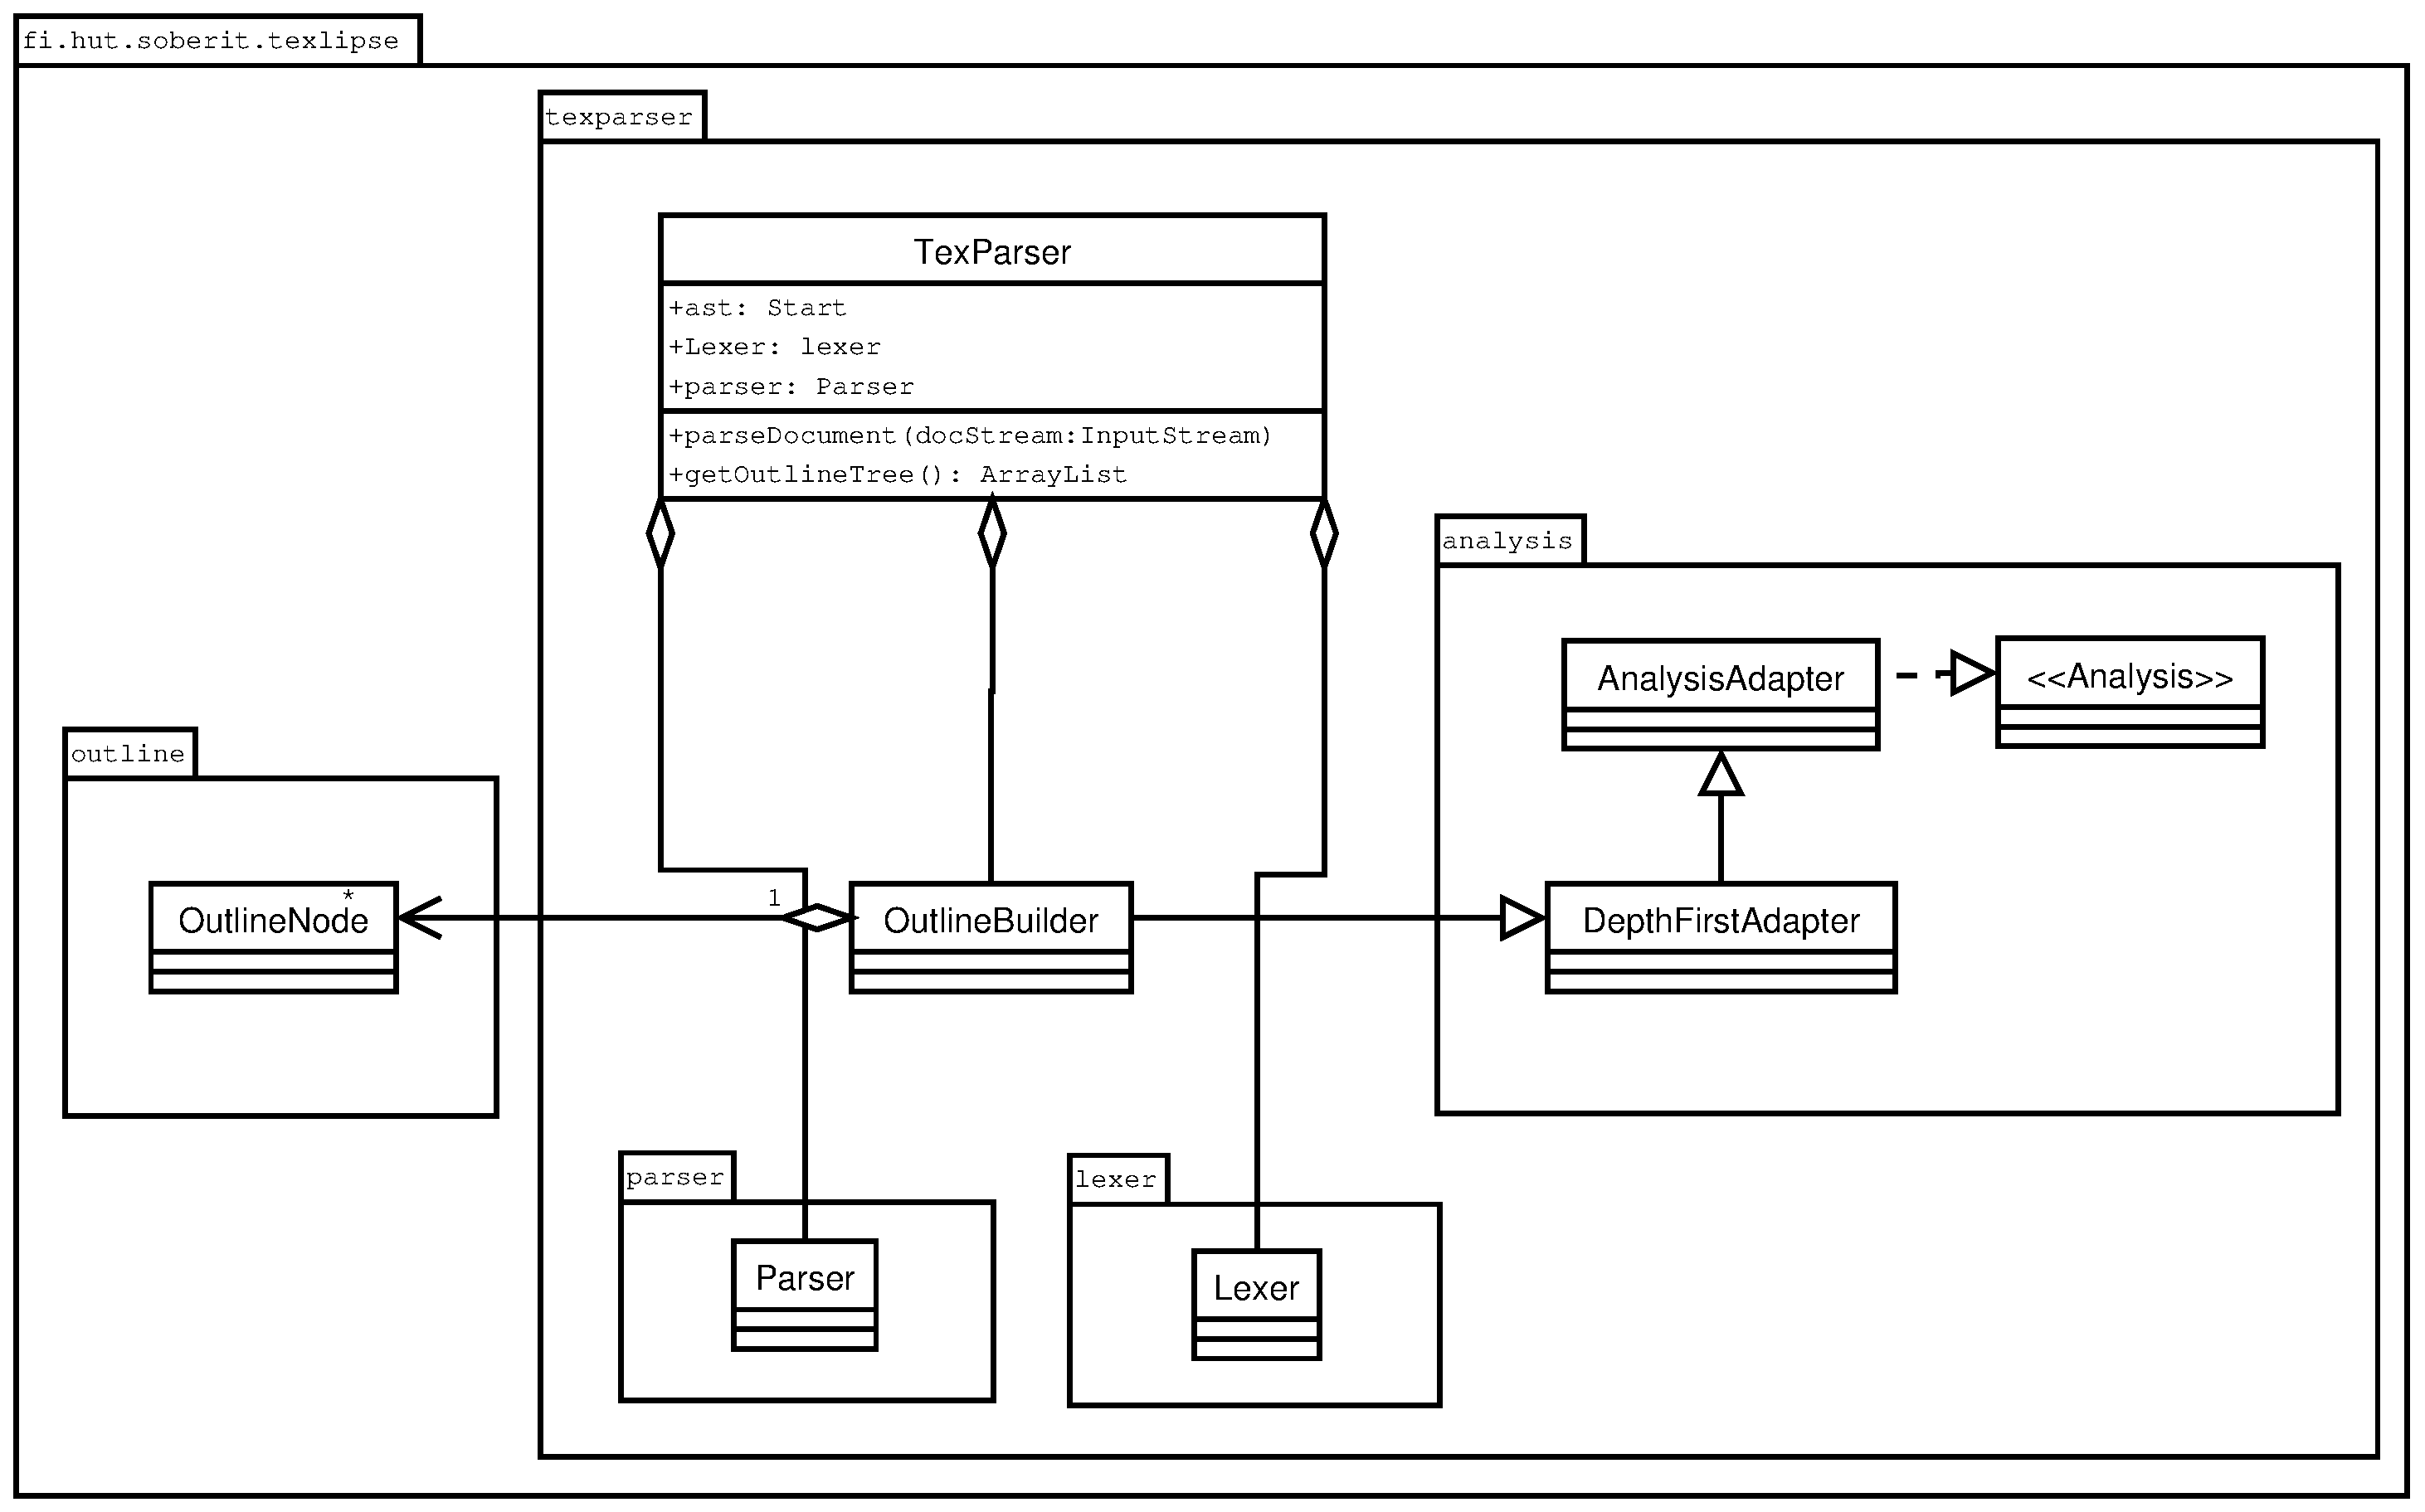
\includegraphics[width=12cm]{images/techtexparse}
% \caption{\LaTeX parser and a depiction of the use of visitors \emph{(To be updated)}}
% \label{fig:parser}
% \end{center}
% \end{figure}

\begin{figure}[!htp]
\begin{center}
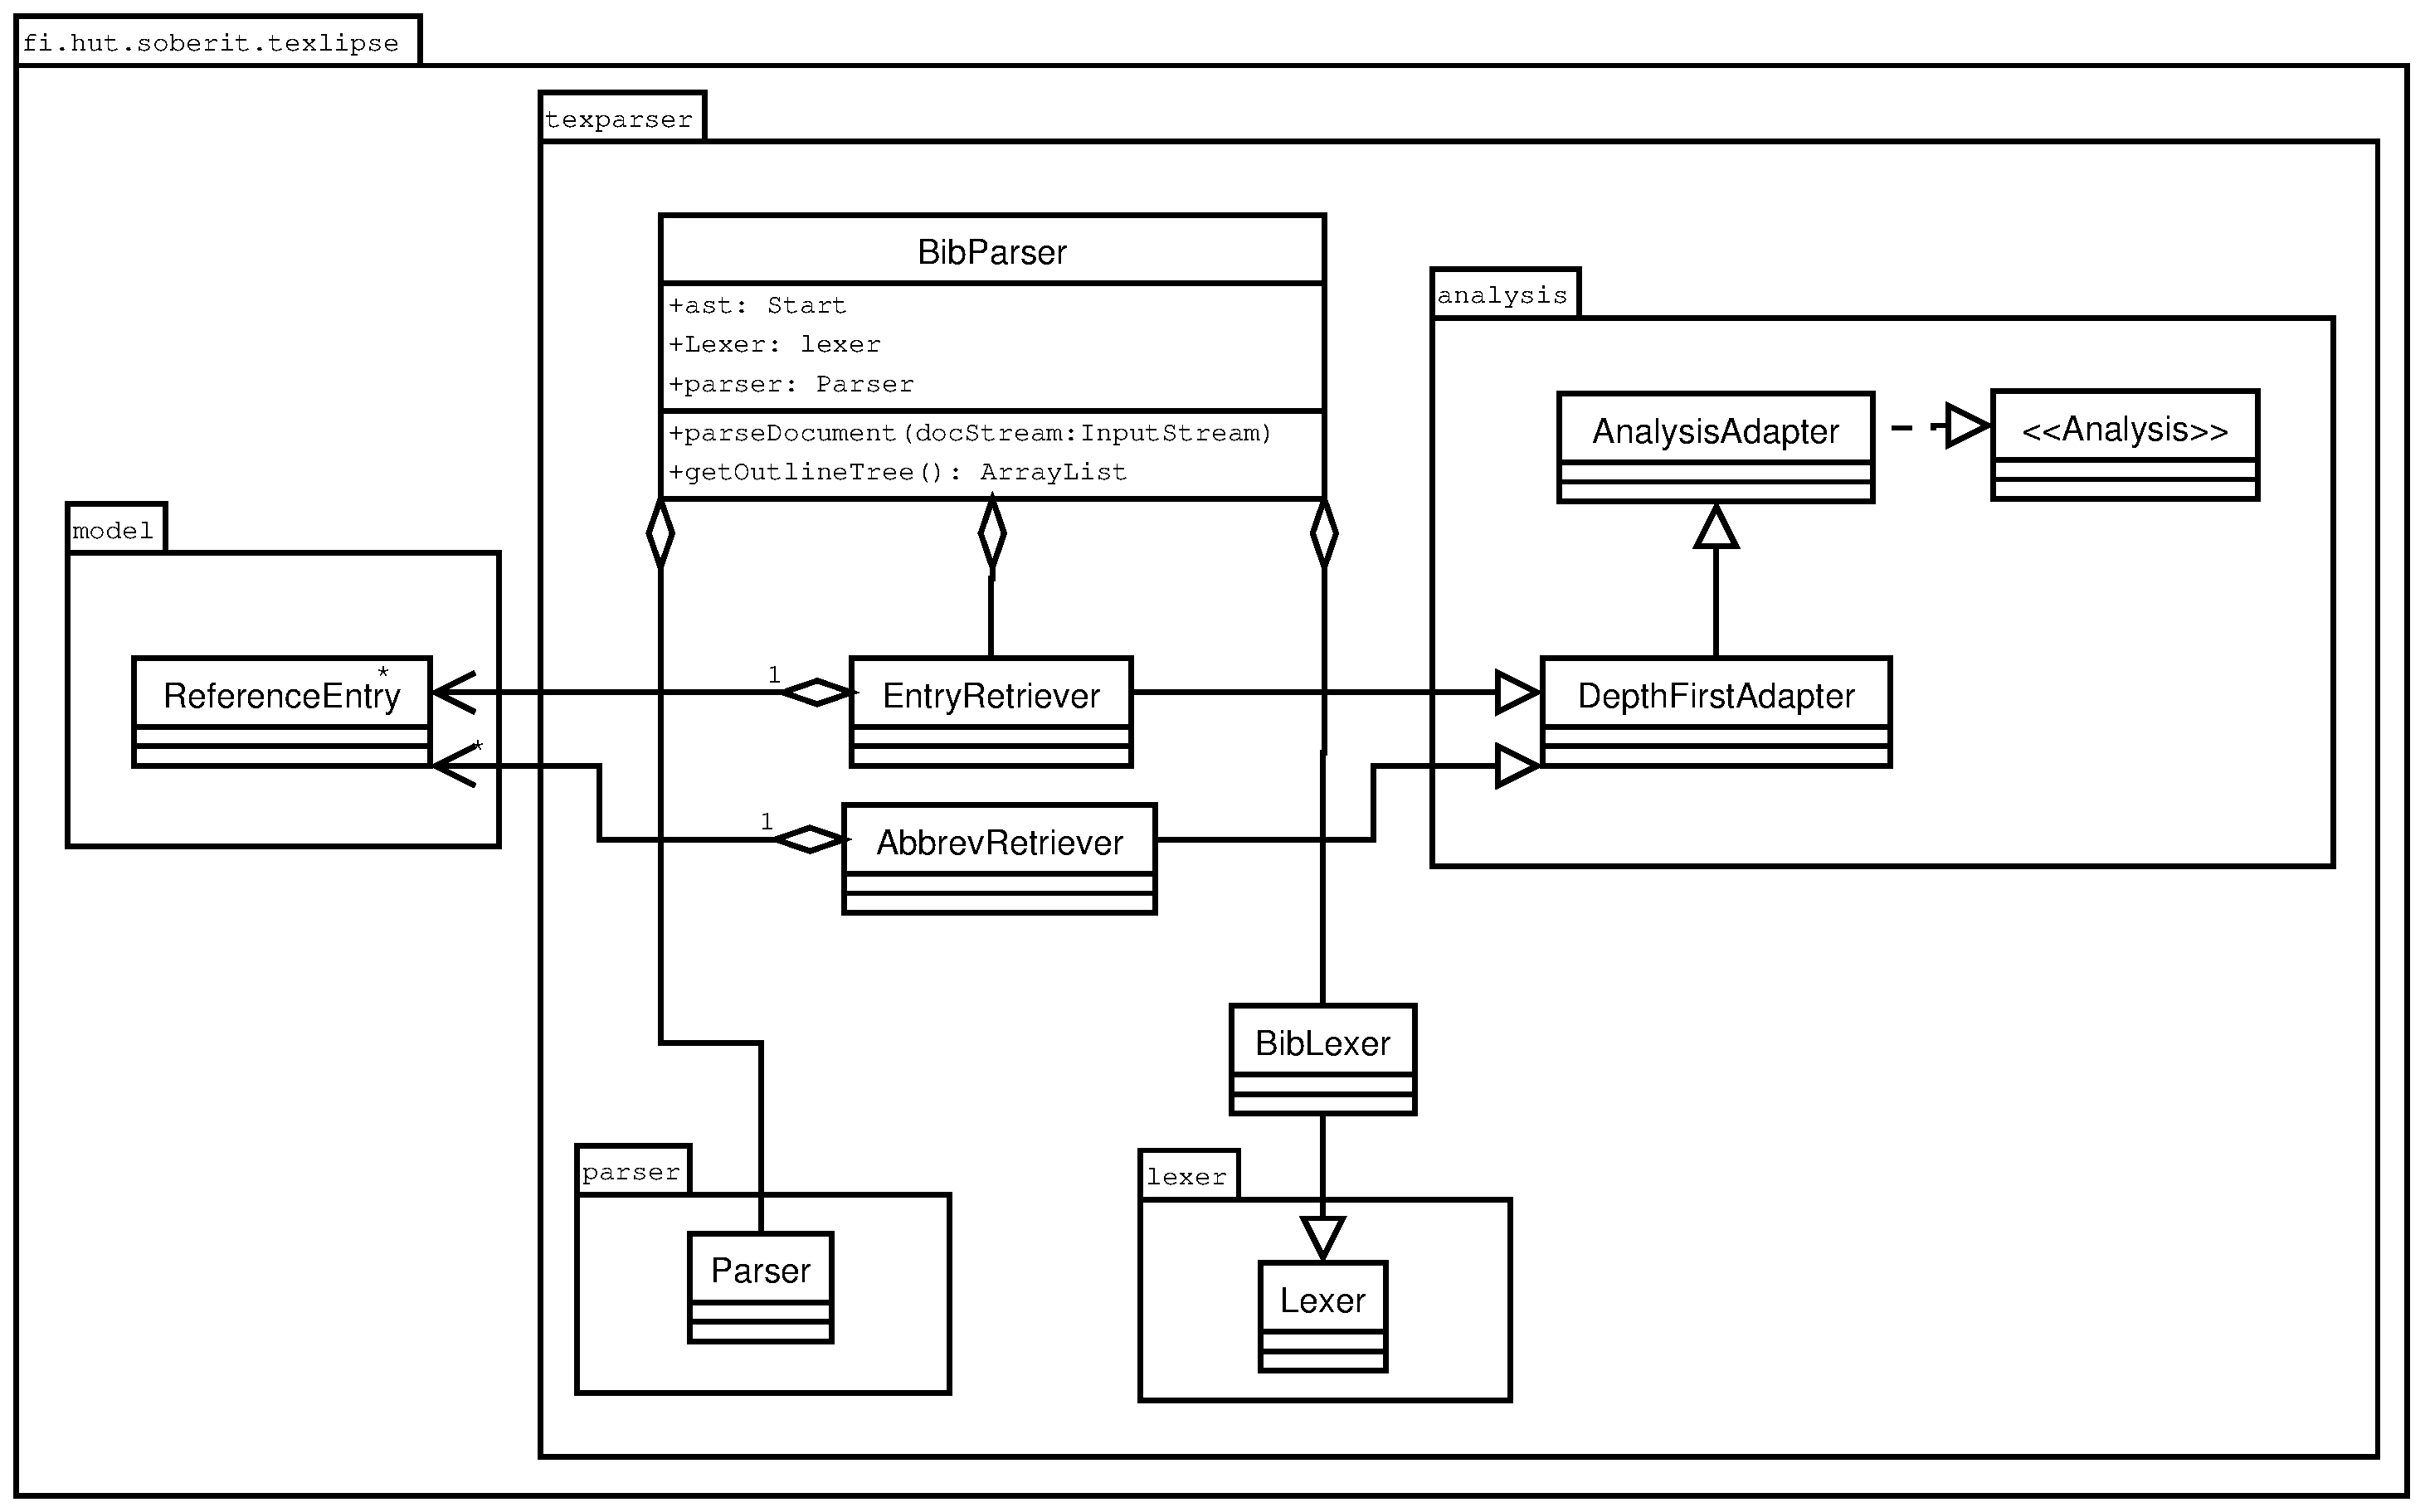
\includegraphics[width=12cm]{images/techbibparse}
\caption{Bib\TeX\ parser and a depiction of the use of visitors}
\label{fig:parserbib}
\end{center}
\end{figure}


The inner workings of the parser-package can be explained by looking at the 
specific case of building an outline tree (or Bib\TeX -completions for the 
\LaTeX -editor --- the process is the same). \texttt{BibParser} in 
Figure~\ref{fig:parserbib} receives a request from the model to parse the 
document and receives a stream (containing the document's contents) to parse. 
It invokes its lexer and parser on the stream, building an AST in the process. 
The AST can now be transformed using the visitor pattern --- applying a visitor 
object on the AST so that the AST calls the appropriate visitor methods of the 
visitor object when the nodes corresponding to the methods are visited. The 
visitor construction is shown in Figure~\ref{fig:parserbib}, as are the 
\texttt{EntryRetriever} and \texttt{AbbrevRetriever} --visitors and their 
inheritance hierarchies (the visitor methods are quite numerous and not 
depicted). When the model needs to update the outline, it requests the outline 
from \texttt{BibParser}, which leads to \texttt{BibParser} invoking the 
\texttt{EntryRetriever} -visitor that constructs the outline, storing the 
result in \texttt{ReferenceEntry} objects, forming a tree (due to the Bib\TeX\ 
syntax, the tree is flat, but the process quite easily permits doing a ``true'' 
tree, as is done with sectioning commands in a \LaTeX\ document). The resulting 
tree is returned to the model and can be directly used in the outline.

The \texttt{AbbrevRetriever} visitor is used to retrieve Bib\TeX\
abbreviations for use in content assist in the Bib\TeX -editor. In this case the
visitor-pattern is quite useful, because the \texttt{EntryRetriever} visitor is
used both by the \LaTeX -editor and the Bib\TeX -editor (but for different
purposes), while the \texttt{AbbrevRetriever} visitor is needed only in the
Bib\TeX -editor and thus it can be easily applied on the AST separately.

This visitor pattern model is employed successfully in parsing Bib\TeX\
documents, but for \LaTeX\ documents we use a more traditional one-pass
parsing approach, mainly due to the lack of benefits in the visitor
approach (Bib\TeX\ has a stricter structure). The issue is
addressed more specifically in Section~\ref{sect:t0.1}.

It's worth noting that the \texttt{analysis}, \texttt{lexer} and
\texttt{parser} -packages are generated by SableCC and are
SableCC-specific; SableCC automatically constructs a visitor interface
and a visitor skeleton implementing that interfaces based on the AST
structure specified in the grammar. The choice of using SableCC, its
advantages and disadvantages are discussed in more detail in
Section~\ref{sect:t0.1}.

% The Bib\TeX -parser is practically identical conceptually --- it
% merely provides different data structures and methods outward and
% internally it implements a different parser.  Hence, it forms a
% separate package.

The use of visitors and an AST enables easy programming and a
relatively clean abstraction of functionality --- our experience thus
far has been that the visitors are fairly easy to program and the
automatically generated grammars provide a lot of convenient
abstraction, e.g. changing the grammar doesn't most of the time imply
refactoring everything. Abstracting the parsers serves to decrease
module coupling and to easily distribute the implementation tasks.
Also, it makes the system easier to understand. However, note the
specific requirements of \LaTeX, discussed in Section~\ref{sect:t0.1}.

The Eclipse plugin framework provides for document scanners implementing a 
relatively easy way to do basic lexing of the document (see 
section~\ref{sect:t1.1} for a use of this). However, while easy to use, these 
scanners are extremely tedious for more complicated grammars due to a lack of 
expressive power and they don't offer the performance and syntactical checking 
advantages of a dedicated parser. One problem with simpler parsing would be 
that the user writes a subsection without a preceding section --- it might be 
valid, but how is the outline supposed to show it? Errors such as this are easy 
to catch with a dedicated parser. We can also check the validity of labels and 
make similar things not possible with simple lexing applications.


\subsubsection{Outline}

The conceptual process of parsing the \LaTeX -document in order to create an 
outline tree was detailed in the previous section. Figure~\ref{fig:outline} now 
shows how the outline view is associated with the rest of the system.

\begin{figure}[!htp]
\begin{center}
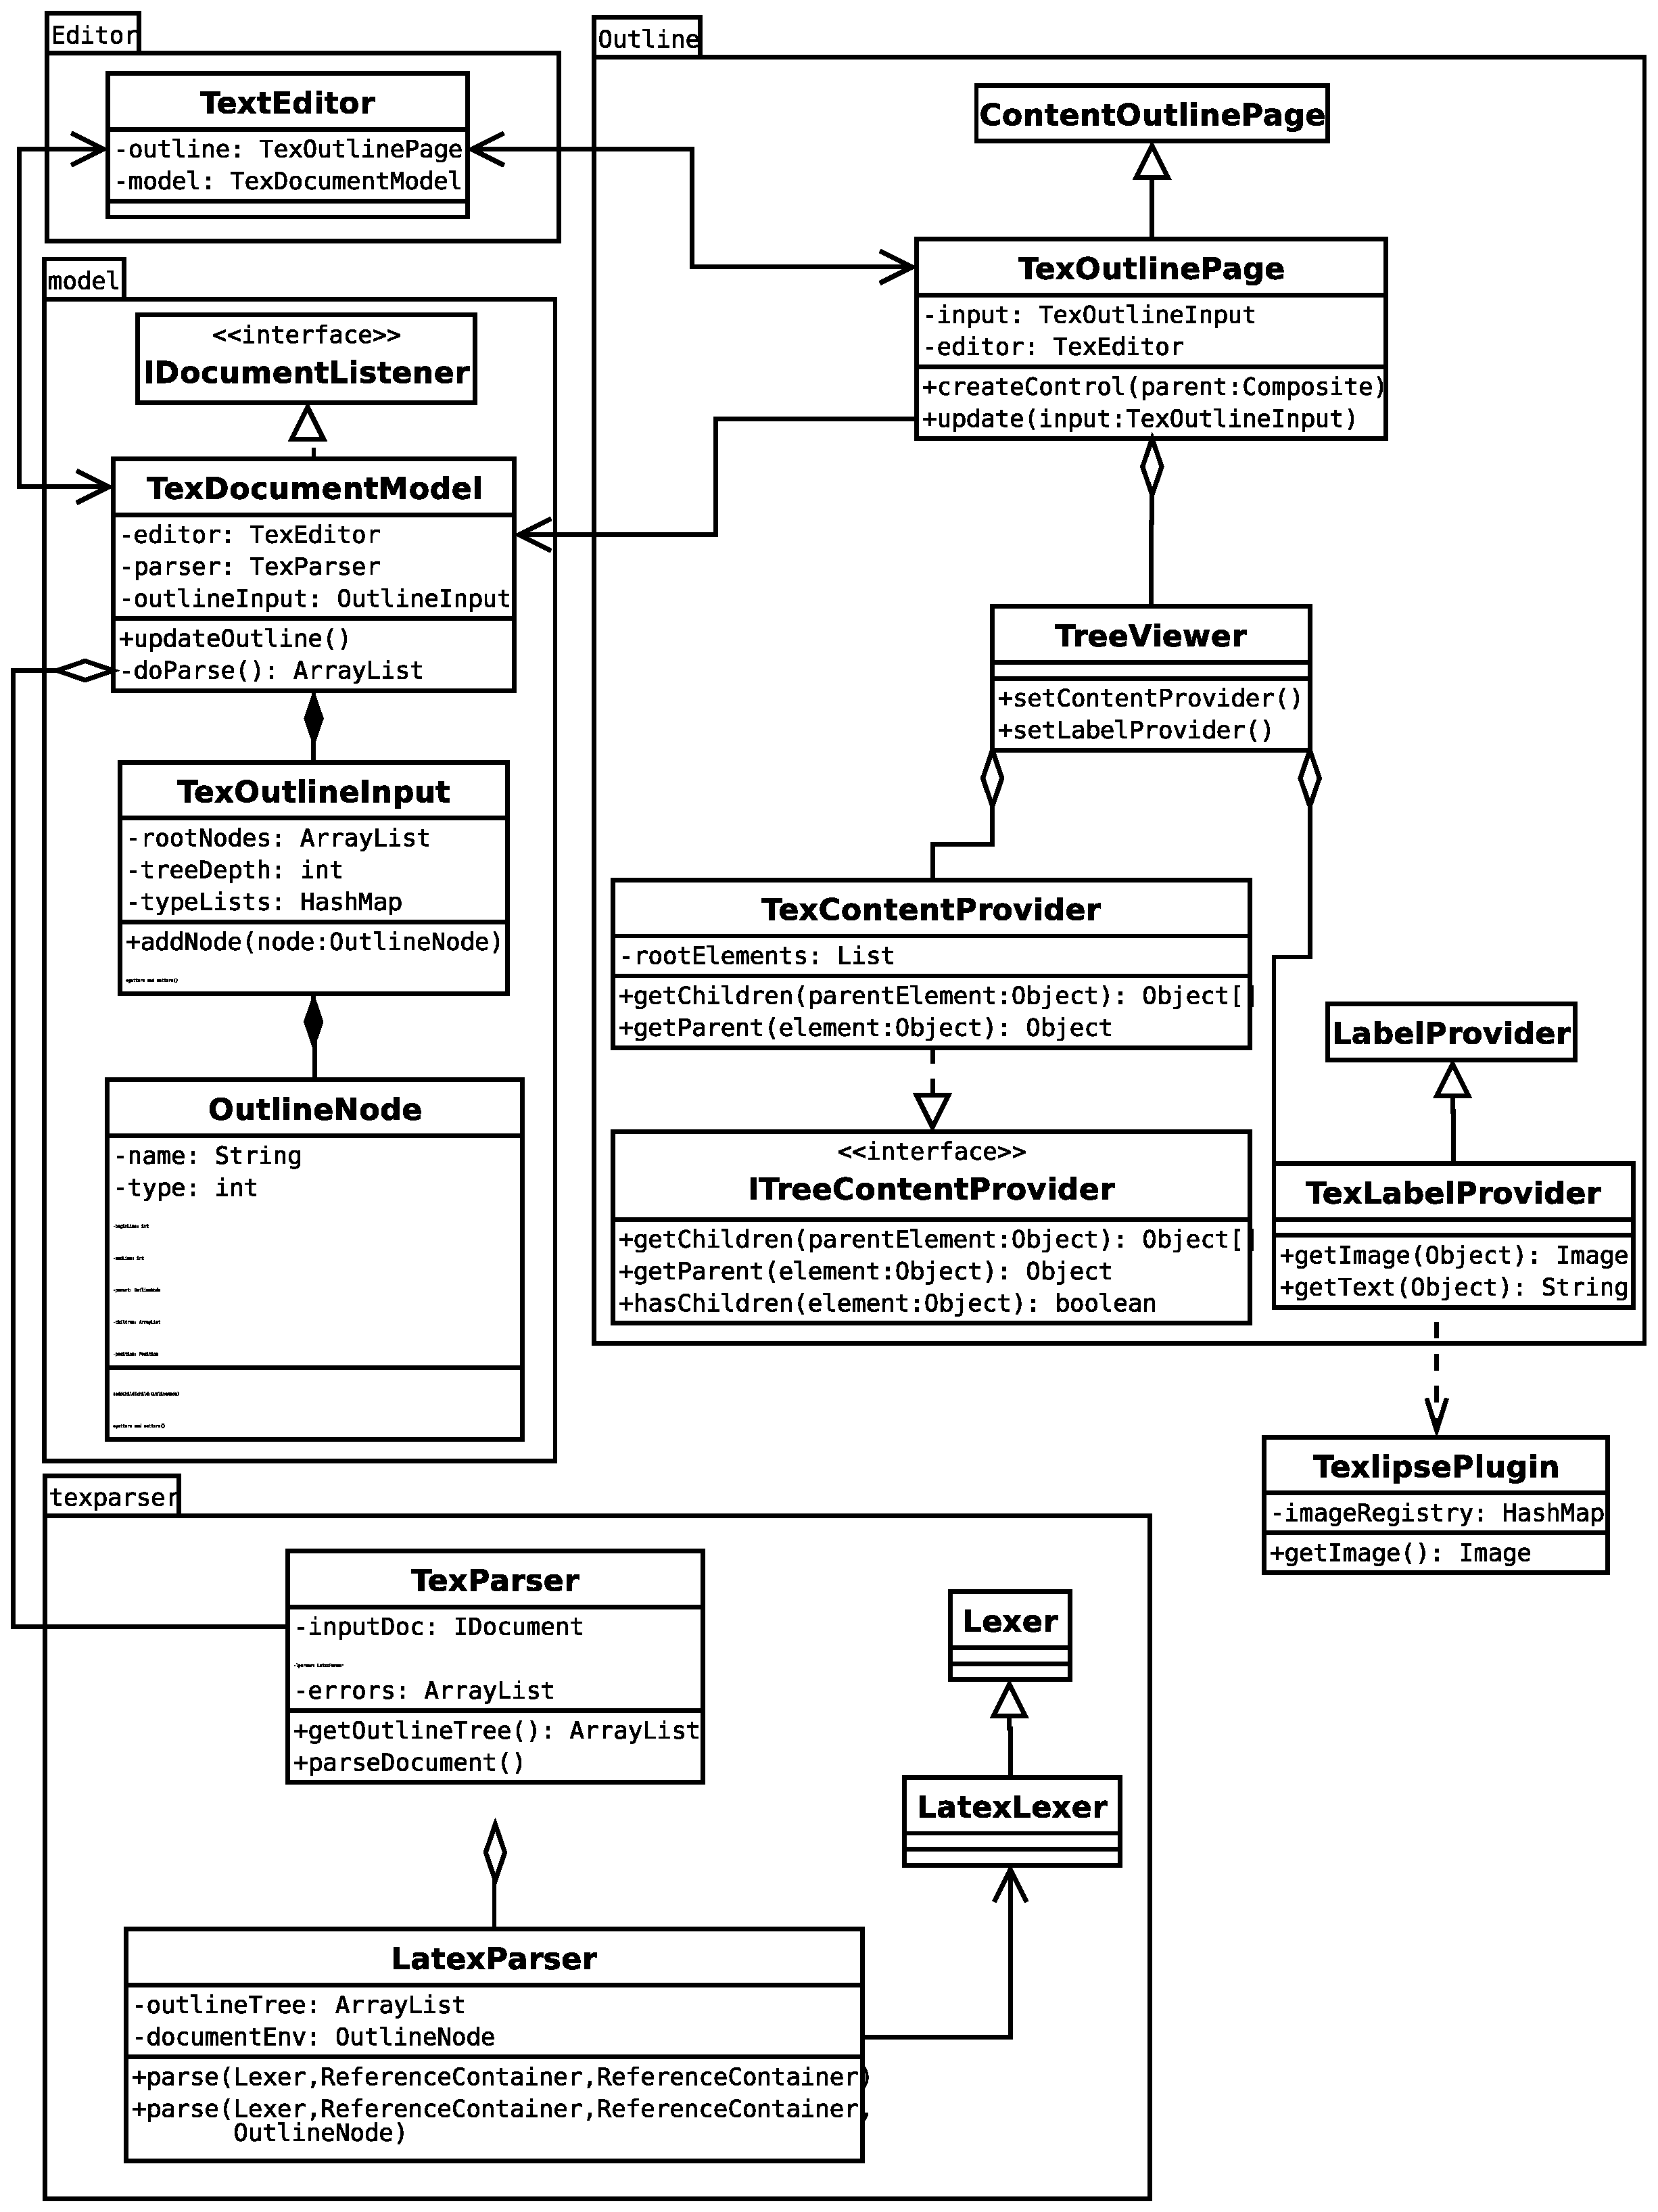
\includegraphics[width=12cm]{images/outline}
\caption{Outline}
\label{fig:outline}
\end{center}
\end{figure}

The way the outline works is described in more detail in 
Section~\ref{sect:t2.1}. What is important to note here is how the 
\texttt{TexDocumentModel} handles calling the parser and holds the tree of 
\texttt{OutlineNode}s representing the outline. The task of the 
outline -package, in turn, is fetching the outline from the model and taking 
care of all tasks in displaying it (this includes displaying the actual tree as 
well as doing such things as choosing the correct icons for each type of node 
in the outline tree to display).


\subsection{External interfaces}

External interfaces used by the \texlipse\ plugin include builder and viewer. 
The builder is the module that invokes the external \LaTeX -program (or the 
likes) and creates a viewable document.

\subsubsection{The Builder}

Figure~\ref{fig:builder} shows the class structure of the builder package and 
the builder's connection to the Eclipse API.

\begin{figure}[!htp]
\begin{center}
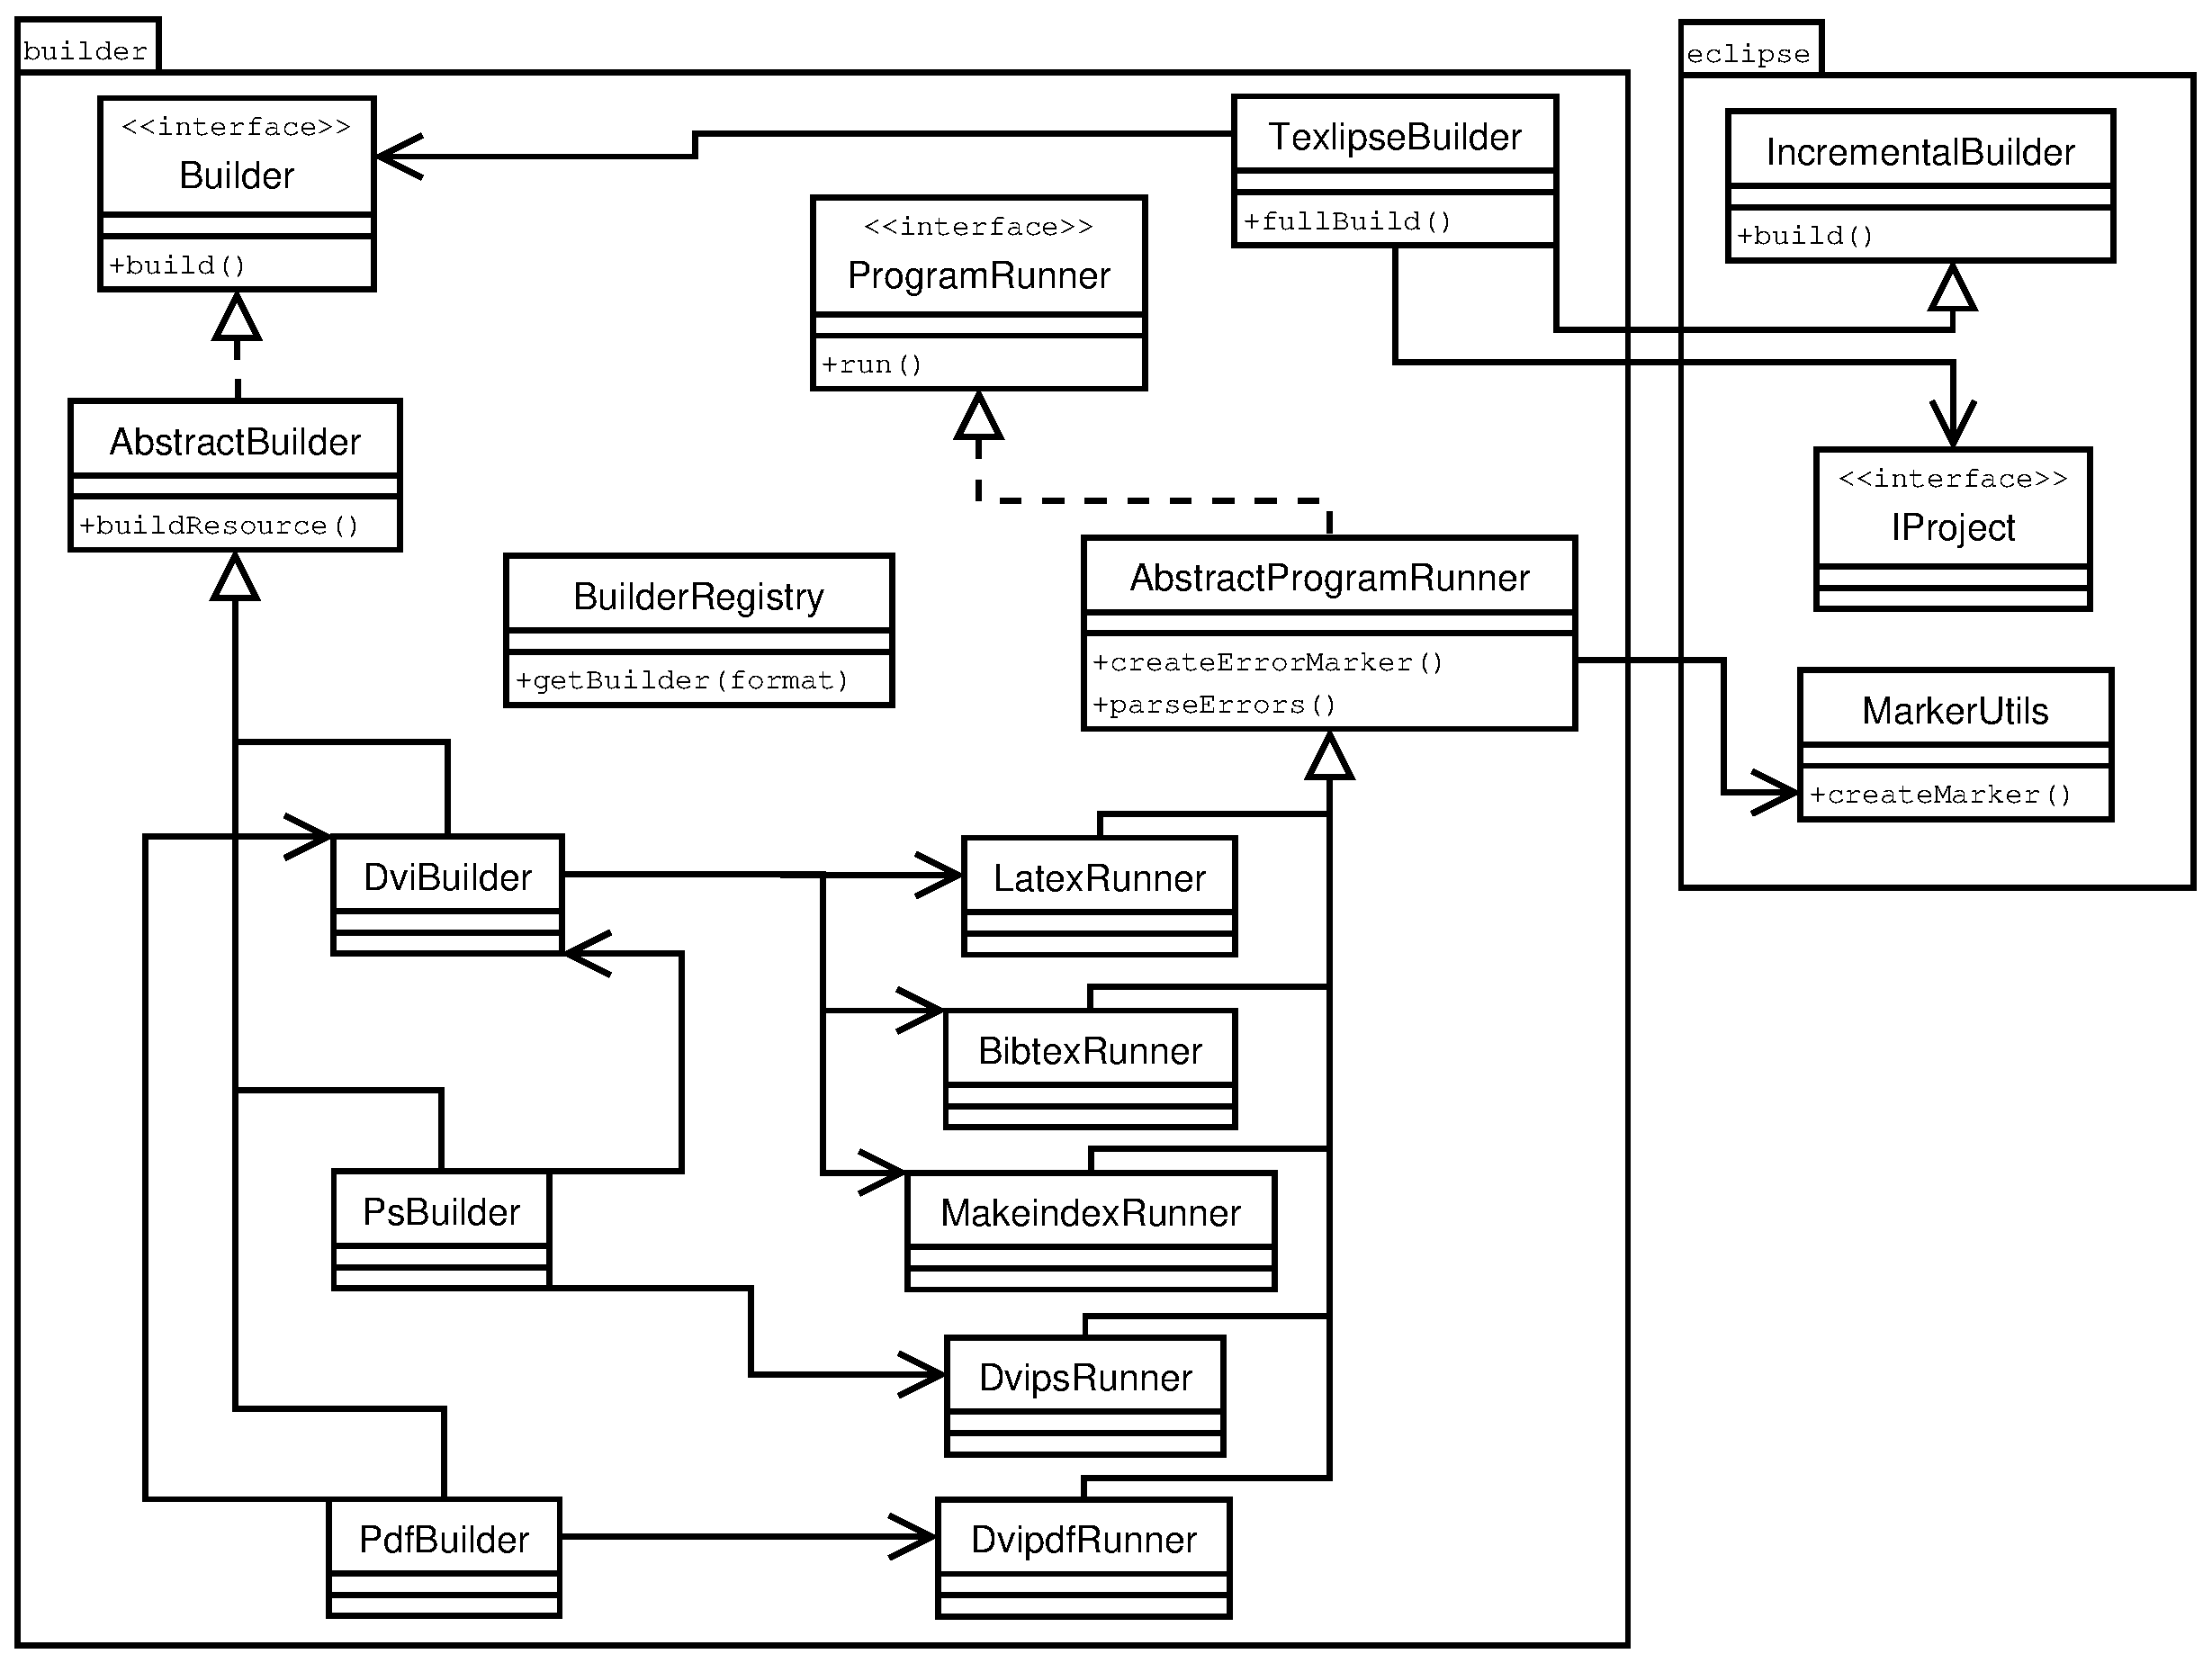
\includegraphics[width=10cm]{images/builder}
\caption{Builder}
\label{fig:builder}
\end{center}
\end{figure}

The builder starts when the user selects \texttt{Project} $\rightarrow$ 
\texttt{Build Project} from Eclipse's menu. Eclipse then instantiates the class 
\texttt{TexlipseBuilder}, because it's defined in the plugin's descriptor file.
\texttt{TexlipseBuilder} does some run-time checks and then consults \texttt{BuilderRegistry}
for an instantiation of the actual builder class (one of the realizations of 
\texttt{AbstractBuilder}). Each builder class is capable of building the input 
\LaTeX -file to one output format. To do this, a builder uses one or more 
program runner classes.

A program runner is an abstract representation of an external program. These 
classes are implemented as realizations of the class 
\texttt{AbstractProgramRunner}. Program runner classes contain methods for 
running the program, stopping the program and parsing errors from the output of 
the program. To display errors, the program runners utilize the 
\texttt{MarkerUtils} class from the Eclipse API.

The paths of the external programs are defined in the \texlipse\ preferences 
page. The output format can be overriden per project so that one project can be 
built to dvi, while another might build to a pdf. Not all supported external 
programs need to be installed. The user needs to configure only those that are 
required for the chosen output format.

At the center of this all is the \texttt{BuilderRegistry}, which holds all the 
actual instances of the builder and program runner classes. The 
\texttt{BuilderRegistry} class itself is implemented using the Singleton design 
pattern (see~\cite{GHJV:despatterns95} for more information). This way, all the 
builder classes can utilize it, and it can still hold an internal global state. 
The \texttt{BuilderRegistry} class provides a method for looking up a builder 
classes for the given output format, and methods to configure program runners. 
The \texttt{TexlipseBuilder} class uses the registry at the start of a build 
process to gain a reference to the correct builder class. The builder classes, 
in turn, use the registry to gain a reference to the correct program runner.


\subsubsection{The Previewer}

Figure~\ref{fig:viewer} shows the class structure of the viewer package and 
viewer's connection to the Eclipse API.

\begin{figure}[!htp]
\begin{center}
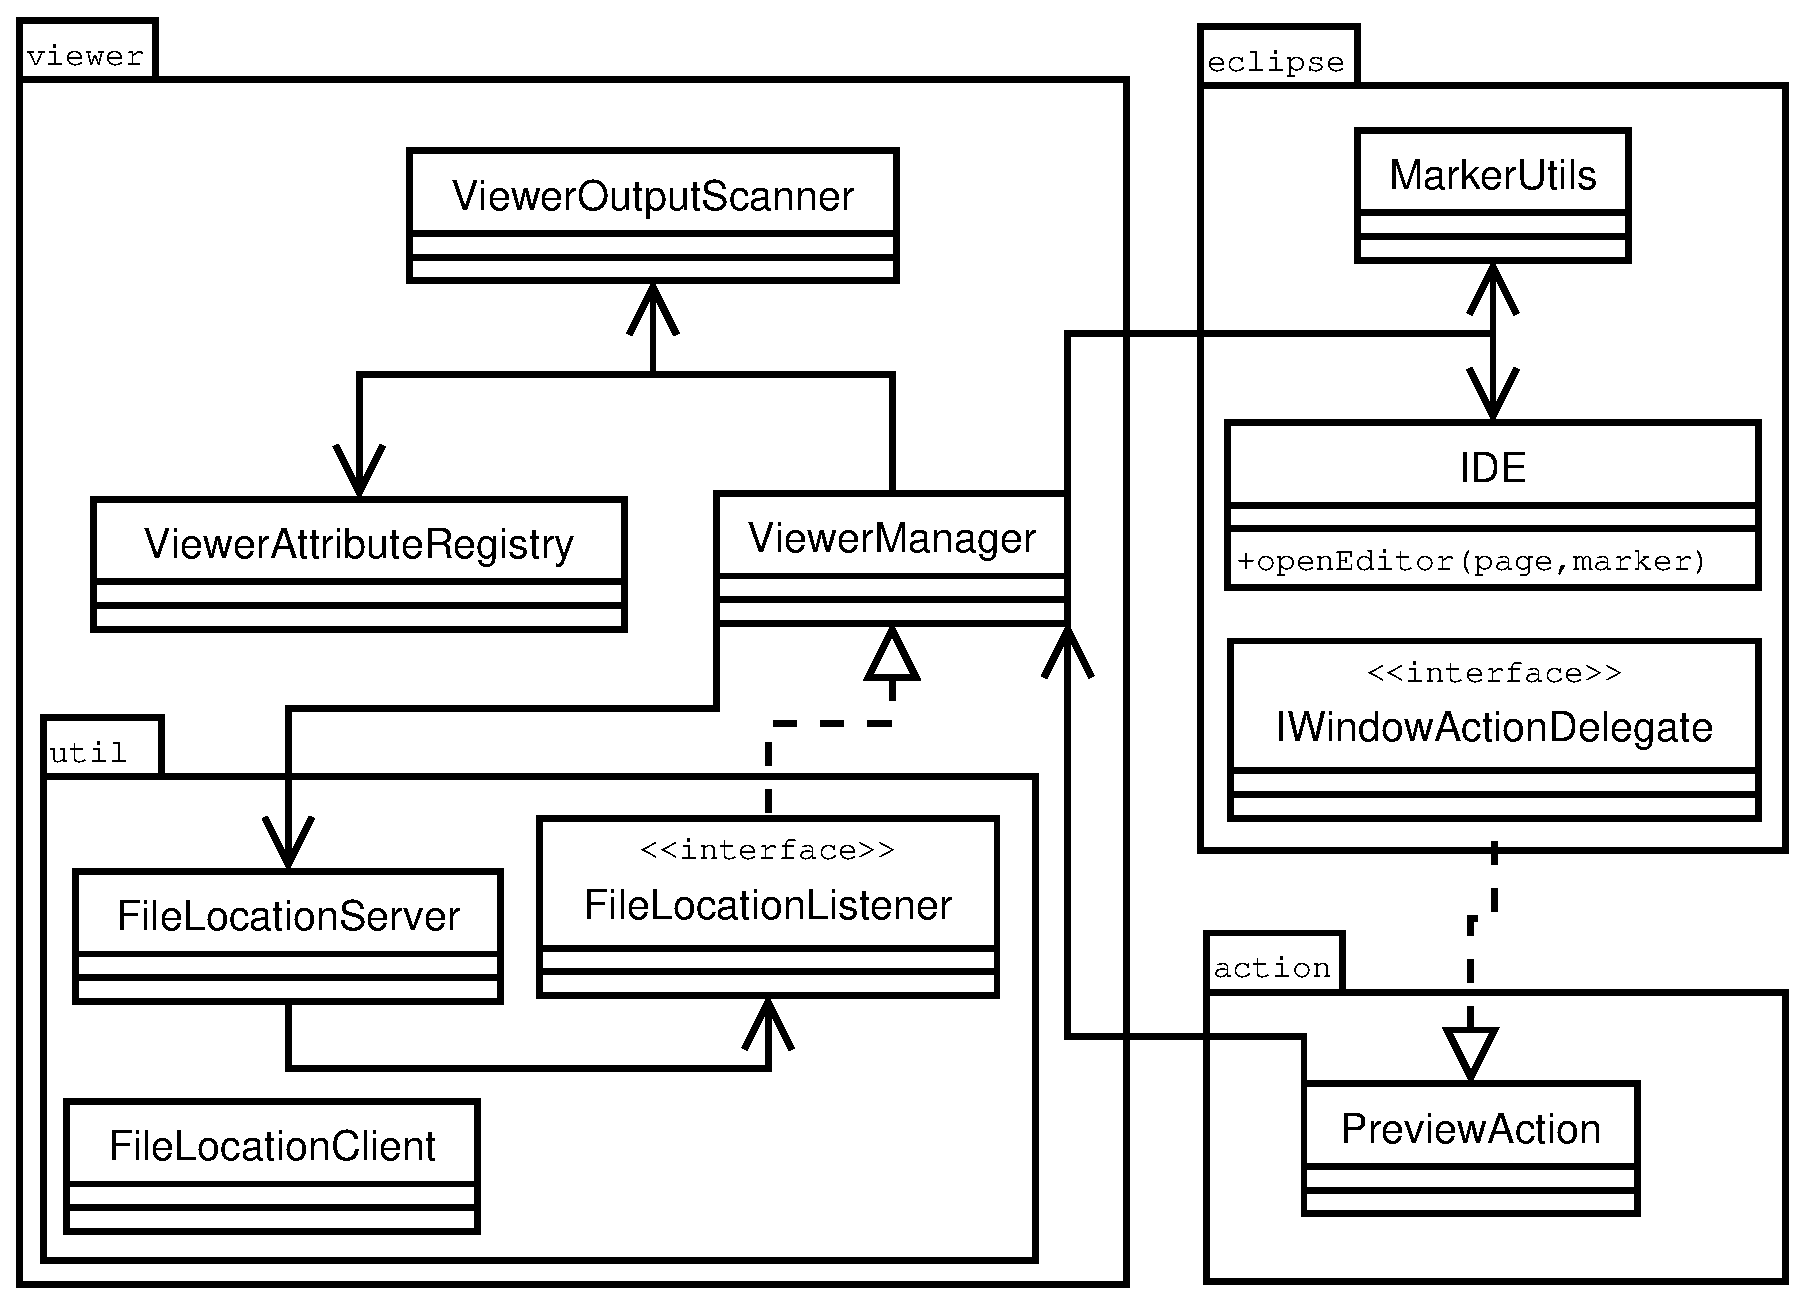
\includegraphics[width=10cm]{images/viewer}
\caption{Viewer}
\label{fig:viewer}
\end{center}
\end{figure}

The viewer can be started by choosing \emph{Preview Document} from the 
Eclipse menu. This causes Eclipse to instantiate the \texttt{PreviewAction} 
class and call its \texttt{run()} method, which calls \texttt{ViewerManager} to 
run the configured external viewer program. The \texttt{ViewerManager} gets the 
viewer program configuration from \texttt{ViewerAttributeRegistry} class, which 
in turn gets it from the plugin preferences. The \texttt{ViewerManager} also 
reads some configuration from the current project, e.g.\ the file name to view. 
\texttt{ViewerManager} creates a running process of the external viewer program 
and, depending on the configuration, instantiates either a 
\texttt{ViewerOutputScanner} or a \texttt{FileLocationServer} or neither of 
them.

The \texttt{ViewerOutputScanner} runs in its own thread and reads the output of 
an external program as long as the program is running. The 
\texttt{ViewerOutputScanner} scans the output for ``filename:linenumber'' 
-strings, which tell that the user wants to navigate to the specified location 
in the source file. The \texttt{ViewerOutputScanner} then creates an 
\texttt{IMarker} object to that location, using \texttt{MarkerUtils} as helper, 
and then calls the Eclipse's \texttt{IDE} class to open the specified file at 
the given marker. This method is supported in Unix systems using the external 
\texttt{xdvi} program.

The \texttt{FileLocationServer} runs in its own thread listening to a certain 
socket. The input for \texttt{FileLocationServer} is similar to that of 
\texttt{ViewerOutputScanner}, i.e.\ ``filename:linenumber'' -strings. This 
method is used on Microsoft Windows systems, where the \texttt{yap} dvi viewer 
is used to preview documents. Yap can be configured to invoke an external 
program when the user wants to navigate from a dvi file to its source \TeX\ 
file. The \texlipse\ plugin provides a client program to invoke, namely the 
\texttt{FileLocationClient}. The \texttt{FileLocationClient} outputs a filename 
and a line number, given as command line arguments, to the socket that the
\texttt{FileLocationServer} listens to. When the \texttt{FileLocationServer} 
receives a valid ``filename:linenumber'' --string, it calls the 
\texttt{FileLocationListener} to navigate to that location. This call 
propagates to the same method in the \texttt{ViewerOutputScanner} as described 
above.



\subsection{Editor functions}

The editor is a central part in \texlipse\ and many of the user requirements 
are related to it. Many of these do not affect other packages or functions, but 
some use the facilities in \texlipse\ already presented in this section.

Document and source code editing are key functions in Eclipse and thus the 
Eclipse plugin architecture offers rich functions for supporting many desirable 
editor functions. An example of a feature implemented within the editor 
framework is syntax highlighting. Syntax highlighting is achieved by using 
existing Eclipse document scanners by giving them rules to match and using the 
syntax highlighting framework. Essentially this is making a simple lexer which 
recognizes certain tokens. These document scanners can be used for other editor 
functions too, such as code folding. However, the expressive power of the 
scanners is limited, so we perform code folding using our own \LaTeX -parser. 
In fact, the document outline tree can be re-used for code folding by 
calculating the document offsets to fold into it. This, in turn, can be 
performed as a side effect when building the outline tree in the parser.

Not all functions can be completely made using the classes and interfaces of 
the Eclipse framework. One such function is code completion. The mechanics of 
code completion is done using the Eclipse framework, but fetching and storing 
the actual completions must be done by hand --- in this case using our 
\texttt{TexParser} and \texttt{BibParser} -parser classes, which can parse the 
documents and construct the completion information. When to complete and with
what must also be implemented, which is done by implementing a completion
processor that determines whether a command, a reference or a template should be
offered for completed, how it should be completed and what are the completion
options offered. The completions options come from the parsers and the model
combines all the possible completions in the projects (e.g.\ from multiple
Bib\TeX -files that are included).


\subsection{Code reuse}

Since \texlipse\ is a plugin, it's already based on a large degree of
reuse, as can be noted from the previous sections. Basic menus and widgets,
syntax highlighting, code completion drawing, etc., is eased considerably
by ready-made components. However, this reuse focus on common editing
tasks and it would be desirable to reuse \LaTeX -specific functionality,
too.

The possibility of reusing large amounts (or even some amount) of code is 
highly desirable, since it would shorten development and testing times.  
Indeed, there exists Eclipse plugins for \LaTeX , among them eTex. However, 
after studying it, we have found the documentation to be practically nil and 
the code to be buggy and of dubious technical quality. Thus, it was not chosen 
as a basis for implementation. Other \LaTeX -editors for Eclipse suffered from 
being very limited in scope --- \texlipse\ has considerably more features 
planned for implementation, several of them being fairly complex. Thus, we 
chose not to use any code from existing \LaTeX -plugins for Eclipse.

There are several practical tools for solving parts of \texlipse's problem 
domain, one of them being JabRef, which is a program for managing references, 
mainly Bib\TeX -databases. However, JabRef uses a hand-coded parser, which is a 
potential software engineering and performance problem, the internal data 
structures are so different than ours that refactoring would be significant and 
on top of it all its license (GPL) doesn't comply well with an Eclipse plugin. 
Due to these reasons, no code from JabRef is used.

For aiding the construction of some \LaTeX -code, some good sources exist.
For Bib\TeX , prof. Nelson Beebe's articles
(see~\cite{Beebe:TB14-4-395-419}) are highly useful and there are many
good books about \TeX\ and \LaTeX , which make designing significantly
easier. So while we don't have the opportunity to reuse code, we have
many ideas to reuse.


\section{Technical specification per implementation task}
\label{sect:techntasks}

\subsection{Make \LaTeX\ parser (T0.1)}
\label{sect:t0.1}

\texttt{Package: texparser}

Define a parser (in EBNF) for a subset of \LaTeX. Specifically, we want to 
recognize sections, references (\texttt{cite} and \texttt{ref} and 
\textbackslash begin \ldots\ end --constructs (i.e.\ environments). The preamble 
should be handled separately, so we can reuse the same parser for \LaTeX 
--files intended only for inclusion, i.e.\ files not containing a preamble and a 
\textbackslash begin\{document\} ... end\{document\} --block.

An easy way to achieve this is to recognize command words and their structure 
(i.e.\ we don't have a subsection without a preceding section) using a parser.  
For generating the lexer and parser from an EBNF description, the tool SableCC 
is used (see \url{http://www.sablecc.org}).

SableCC was chosen over JavaCC and ANTLR primarily because it doesn't require 
entering action code into the grammar specification and the CST to AST 
transformation syntax is concise and clear. In contrast, JavaCC and ANTLR 
require extensive action and tree transformation code to be embedded into the 
grammar, resulting in messy, difficult to debug, difficult to maintain and hard 
to read code. (The problem is somewhat compunded by the action syntax that 
JavaCC uses --- Lex seems to be more ``C-like'' in its syntax than JavaCC is 
``Java-like'' in its syntax.) SableCC solves this problem with clean grammar 
files and encouraging the use of a visitor pattern to transform the 
automatically generated AST for different uses. In \texlipse, one such use is 
to extract all the data necessary to make an outline and present it in a tree 
structure.

There is, however, one problem with this approach: \TeX\ and Bib\TeX\ contain 
constructs of type $A \rightarrow \{ A \}$, which are not recognizable by 
regular expressions but are with context-free languages. 
Beebe~\cite{Beebe:TB14-4-395-419} solves this with action code in the 
Lex-definition. This would be possible in, for example, ANTLR, but not directly in 
SableCC. The SableCC object-oriented framework does, however, offer the 
possibility to subclass the lexer and implement the \texttt{filter()} method, 
where such action code can be embedded (somewhat like a template method 
--pattern~\cite{GHJV:despatterns95}). There are other ways to solve the 
problem; the constructs can be recognized in the parsing phase and then 
concatenated (in practice, we want to handle Bib\TeX -strings of the form \{ 
... \{ ... \} ... \} as one string) by visiting the AST. In practice, 
subclassing the lexer is very performance efficient and makes the later stages 
much simpler. The only drawback is that the lexer is not fully understandable 
from the SableCC definitions alone.

Other reasons for choosing SableCC was the support for unicode lexers (which 
can be useful in the near future) and the fact that it makes an LALR-parser, 
not LL(k) as does JavaCC and ANTLR. The latter generators suffer practically no 
penalty in terms of expressive power by using predicates, but these come with 
significant penalties in maintainability and debuggability. Their 
AST-generation is more cumbersome, requiring use of separate tools, and they 
don't have mechanisms to check for the validity of the formed AST, leaving this 
to the programmer unlike SableCC. For further comparison and details of 
SableCC, refer to~\cite{Gagnon:mth-98}.

In practice, however, further study of the syntax and possibilities of
\TeX\ and \LaTeX\ and the requirements of making \texlipse, it became
clear that the fancy AST generation with visitors is not that advantageous
for \LaTeX\ as it is for Bib\TeX\ or programming languages. We could perform
all the necessary functions (outline building, label and command extraction,
etc.) in a single pass, making the parsing simpler and faster. In particular,
\LaTeX\ doesn't have strict semantics in the way that programming languages 
have, so we would simply have had a grammar defining words interspersed by 
commands. Also, the possibility to define own commands and the 
bad-but-not-forbidden --constructs possible in \LaTeX\ make LR parsers less
useful. The problems are further compounded by the way Java uses memory, method
bindings being dynamic and the lack of flexibility in static configurations,
making performance a much more significant issue than with C or C++.

The only drawback with hand-coding the parser (the lexer is naturally
automatically generated) was the somewhat massive parser class. However,
due to the relative simplicity of the parsing task and the fact that the
visitor would be equally complex but just have more methods, this
approach was pursued.

% The framework for parsers in \TeX lipse is explained in 
% Section~\ref{sect:techparse}.

See~\cite{Aho:CPT86} and~\cite{Knuth:j-IC-8-6-607} for basic information on 
parsing and particularly LR-parsing. See \cite{Knuth:texprogram86} for 
information on how the original \TeX\ parses its syntax.


\subsection{Syntax highlighting, basic case (T1.1)}
\label{sect:t1.1}

\texttt{Package: editor}

Syntax highlighting can be made easily by using a simple lexer/DFA that 
recognizes \TeX 's keywords and colorizes them. This can conveniently be done 
using Eclipse's built-in scanner-facilities, which can be given rules and then 
scan the document automatically. The highlighting itself is easy, but the 
expressivity of the premade rules is quite limited, so we need to make our own 
rule-classes.


\subsection{Code folding (T1.2)}

\texttt{Package: editor, model, texparser}

Eclipse provides a framework for code folding and the foldable sections can be 
recognized either with the document scanners (as in Section~\ref{sect:t1.1}) or 
the outline tree made by \texttt{TexParser} can be used. For the foldable 
sections, their positions in the document must be stored. We do this in the 
\LaTeX -parser by simply reusing the document outline tree that we need to 
create for the outline. The same positions needed in the outline are used as 
positions for code folds.

The actual code folding is largely done by Eclipse-classes, but we need to 
create the folding annotations, which means traversing the outline tree and 
making suitable annotations from each node to be placed into the code folder. 
This is somewhat tricky, since the folder has a flat datastructure, which makes 
it somewhat difficult to determine which annotation in the folder corresponds 
to which node in the tree (e.g.\ for maintaining folding across a save).


\subsection{Automatic indentation (T1.3)}
\label{sec:t1.3}

\texttt{Package: actions, editor}

Classes for supporting automatic indentation are provided with Eclipse. The 
indentation strategy can be determined by using the document scanners mentioned 
in Section~\ref{sect:t1.1}. In addition to this, an entirely own logic of when 
and how much to indent is made. It bases it's decisions on the previous lines, 
as do practically all other Eclipse editor plugins.


\subsection{Make Bib\TeX\ parser (T1.4)}

\texttt{Package: bibeditor}

The Bib\TeX\ grammar is more strict than \TeX\ and merely defines an entry 
format to specify bibliography entries. Due to this, it is fairly well suited 
to LALR-parsing.

The grammar is made using SableCC, which creates an AST automatically. 
Section~\ref{sect:t0.1} explains the rationale behind using SableCC. The 
framework for parsers in \texlipse\ is explained in 
Section~\ref{sect:techparse}. It is worth noting that the framework permits 
adding support to \texlipse\ for some other bibliography format elegantly, 
which might be desirable due to the problems with Bib\TeX\ (problems recognizing 
string literals, somewhat badly defined comment syntax, etc.)

The Bib\TeX\ grammar is not very well defined (or designed), so some .bib files 
using uncommon syntax might not parse correctly (use prof.\ Nelson Beebe's tools 
for pretty printing them). However, the \texlipse\ Bib\TeX\ parser recognizes 
all the common Bib\TeX -conventions. The grammar is based pretty much on 
Beebe's observations in~\cite{Beebe:TB14-4-395-419}.

It should be noted that LR-parsing is considered significantly harder to debug 
than LL, but having done extensive testing with SableCC for use in Eclipse we 
have not found this to be a problem, in part due to the excellent automation 
and error-detection of SableCC.

See~\cite{Aho:CPT86} and~\cite{Knuth:j-IC-8-6-607} for basic information 
on parsing and particularly LR-parsing.

See~\cite{Lamport:LDP85} and \cite{Patashnik:Bib-TUG-03-1} for further 
information about the Bib\TeX\ format.



\subsection{Code completion (content assist, T1.5)}
\label{sec:t1.5}

\texttt{Package: editor, model, texparser and bibparser}

For code completion we need both the user's Bib\TeX -files' contents and the 
labels defined in the document. The .bib -files are parsed at startup and when 
saving the .bib -files. What bib-files to parse are read from the document's 
\verb+\bibliography+ -command. The labels are retrieved whenever the project 
documents are parsed. They are stored into two similar datastructures (one for 
completing \texttt{ref} and the other for \texttt{cite} commands) in the model, 
from which the editor's code completion classes can fetch them. The data 
structure containing the completions is stored so that every model in the 
project can access it and it supports partial compilation so that reparsing 
one bib-file doesn't require reparsing all the others to enable completion. 
Thus, performance can be increased by splitting the .bib -files.

The Eclipse plugin framework provides a number of classes and interfaces for 
supporting code completion in the editor view.

Storing the completions in a linear structure (array) and searching it takes 
$O(n\cdot m)$ time, where n is the size of the array and m is the time for 
partial matching a string. With a B-tree, the time is $O(\log n)$, but 
constructing it is more difficult and the constant terms dimnish the advantage. 
A third approach is to make a sorted array and use modified binary search to 
fetch the entries. The modified binary search (to fetch a range of values) is 
still $O(\log n)$ and sorting can be done in $O(n\log n)$ time, but this is 
only done after a modification on the reference source document. The constant 
terms are smaller than with a B-tree and the implementation is much simpler, in 
part since we can use Java's built-in mergesort.

Performance must be evaluated to make hard conclusions. In practice, the third 
option was implemented based on theoretical merits and seems to provide very 
good performance.


\subsection{Template mechanism, user defined templates (T1.6, T1.7)}

\texttt{Package: templates, editor}

There are two different types of templates --- project templates and editor 
templates. The former ones are whole \LaTeX\ documents (they can be compiled 
directly), which may be used when a new \LaTeX\ project is created (i.e.\ the
selected template is copied to the main project file as it is). The latter 
templates are smaller pieces of \LaTeX\ code (for example \emph{lists} or 
\emph{theorem \& proof} structures) that can be inserted anywhere into the 
document.

The user can define her own templates, both project and editor. The system has 
two directories for storing project templates (namely, \emph{<TeXlipse 
plugin>/templates/} and a template directory under teh workspace -directory's 
\emph{.metadata/.plugins} -directory), in which the templates reside. Both
template systems have separate mechanisms, so they will be explained separately.

The user can freely add her own project templates and add them to the system's 
\LaTeX\ template directory (if she has the rights to do it) or use the editor 
action of saving a template, in which case the template is saved under the 
workspace -directory mentioned above. The project creation wizard (see
Section~\ref{sec:t4.1}) supports these temlates by presenting a list of
available templates (both user and system) and copies the contents of the chosen
template directly into the new main \LaTeX\ document that is created.

The editor template handling is really a special case of using content assist. 
Thus, editor templates can be used as content assist is used and they can be 
edited, exported and imported in the Eclipse Preferences. Eclipse provides a
ready made mechanism both for storing and for retrieving the templates, which
requires a relatively small amount of code to activate. For inserting editor
templates, the content assistant framework detailed in Section~\ref{sec:t1.5} is
invoked. It determines what kind of completion is done and if a template
completion is done, it requests teh completions from the template manager. The
template manager is really an adapter between the content completion processor
and Eclipse's template mechanism. It fetches the available templates and
computes the allowed completions. Unlike the reference and command completions,
this is done in linear time due to apparent restrictions placed by the Eclipse
framework, but since the amount of templates available is not usually that large
this should not be a problem.


\subsection{Commenting blocks (T1.8)}

\texttt{Package: actions}

Blocks (region in emacs-parlance) can be commented by inserting a 
\% -sign at the start of each line in the block. They can be removed 
by reversing the process and ignoring leading whitespace.

Alternatively, \verb+\begin{comment}+ and \verb+\end{comment}+ 
-commands can be used, but noticing them is not as obvious
(especially if one has to use a non-highlighting editor due to
some reason), so using the \% -syntax was chosen.


\subsection{Annotations for errors (T1.9)}

\texttt{Package: model, texparser}

We use the built-in annotation facility and place markers on offending
lines. Offending lines can be recognized by parsing the document and
examining the document references' symbol tables.

Offending lines are also recognized from the output of the build process.
The builder parses the output of \LaTeX, Bib\TeX, and other document
builder programs, which report errors about the source documents.


\subsection{Matching parens (T1.10)}

\texttt{Package: parenmatcher}

See Section~\ref{sect:t1.1}; essentially this is done with the same
tools and it uses facilities provided by Eclipse. Eclipse provides and interface
called \texttt{ICharacterPairMatcher}, whose concretizations can be activated in
an editor to enable matching of pairs. In \texlipse, it is implemented and used
so that \{, \}, [, ], ( and ) are matched.


\subsection{Word counter (T1.11)}

\texttt{Package: actions, texparser}

The word counter action enables counting the number of words in the
selected region, taking into account the special characteristics of
\LaTeX -source. Due to this, this is most conveniently performed by
making a simple parser that gets its input from the \LaTeX -parser
(see Section~\ref{sect:t0.1}) and the determines how to count based on
the token encountered.

\subsection{Line wrap (T1.12)}

\texttt{Package: actions, editor}

The line wrapping functionality is an extension to the indenting functionality
specified in Section~\ref{sec:t1.3}. Basically, it has two alternative modes (in
addition to disabling wrapping altogether): soft wrap and hard wrap, that can be
chosen from the plugin preferences.

The hard wrap uses normal means of string manipulation to wrap text into a given
line width. It does take into account some special conditions, such as being
inside an indented region and the typed area being succeeded by a lone command
(e.g.\ \verb+\bibliography+ or \verb+\section+).

Soft wrapping is implemented by enabling it from Eclipse's standard text viewer
interface. However, Eclipse 3.0 has a bug which causes the vertical bar
(containing error annotations and code folding markers) to be displayed
incorrectly when soft wrapping is enabled. Thus, the soft wrap option in the
preference currently has a warning text. In addition, the soft wrapping
mechanism is rather slow and the hard wrapping mechanism used is significantly
faster.


\subsection{View the outline (T2.1)}
\label{sect:t2.1}

\texttt{Package: outline, model, texparser}

The outline shows the outline of the document being edited. (See also 
Section~\ref{sect:archdm} for an overview of the document model.) The outline is 
displayed in a tree structure similar to that of the Java editor of Eclipse. 
For creating the tree structure, a TreeViewer viewer will be used. The viewer 
allows us to avoid working directly with SWT widgets and their event handling. 
Instead, we can concentrate on providing the model of the outline.

The TreeViewer itself does not know much about the contents of the outline. It 
retrieves the elements of the outline from \texttt{ITreeContentProvider} and 
uses a \texttt{LabelProvider} to get a presentation (text and icon) for each 
element. Thus, we implemented a \texttt{TexContentProvider} and a 
\texttt{TexLabelProvider}.

Parsing the document to form the outline tree is handled by the 
\texttt{TexDocumentModel} and the underlying \texttt{TexParser}. The 
\texttt{TexDocumentModel} provides a tree structure for the 
\texttt{TexContentProvider}. The elements of this tree contain the name, type 
and position (start line and length of the part of the document it covers) of 
the element.

When the user changes the document, the \texttt{TexDocumentModel} is changed too. 
If needed, the model triggers the outline to be updated. Thus, the outline itself 
does not actively monitor whether the document is changed or not.

For filtering the elements of the outline, a filter was implemented in the 
class \texttt{TexOutlineFilter}. It is used to specify which document sections 
(preamble, parts, chapters, sections, subsection, subsubsections, paragraphs 
and enviroments) should be visible in the outline.

For saving the state of the outline when an update happens, the names of the 
elements are used. Obviously this is not the optimal solution. A much better 
solutions would be to use the \texttt{position} --field of the 
\texttt{OutlineNode}. Unfortunately, we could not get this to work. The 
positions of the nodes of the old outline were not updated by the Eclipse 
platform, and thus comparing them to the Positions of the new nodes was 
worthless. There is also some discussion about this on the Eclipse forums, but 
no real solution seems be available.

Using the names when saving the state of the outline causes problems when the 
outline has many nodes with the same name. In general, only the state of the 
first element with the same name is saved. The problems are purely visual 
though, and they do not affect the actual document in any way.

The underlying reason for the problems with saving the state of the outline is
the fact that we always reparse the whole document and create a brand new
outline tree, instead of parsing the changed part of the document and only
updating the tree where necessary. However, partial parsing and more
intelligent partitioning was beyond the scope in project leading to \texlipse\
1.0.



\subsection{Basic outline navigation (T2.2)}

\texttt{Package: outline}

When the user selects an element in the outline view, the editor is focused on 
that element. Implementing catching of the selection event and refocusing the
editor was quite straightforward.

However, after discussing with the customer we decided not to implement editor 
to outline navigation, i.e.\ making the outline selection follow the editor 
cursor position. It could be implemented, but would require implementing a 
special search data structure in \texttt{TexDocumentModel}, and was considered 
not worth the effort.


\subsection{Copy/paste and drag'n'drop in the outline (T2.3, T2.4)}
\label{sect:t2.3}

\texttt{Package: outline}

The outline copy/paste and drag and drop support enables the user to manipulate 
the document by copying, cutting, pasting or dragging and dropping the elements 
of the outline tree. Copy/paste and drag and drop are very similar operations
and their implementations are also very similar. The following text mostly 
discusses copy/paste, but it largely applies to drag and drop too.

The copy/paste support of the outline is text based. This means that 
manipulating the elements of the outline will actually manipulate the text of 
the document directly. After the manipulation, the outline is rebuilt to 
reflect the changes.

When performing a paste operation, the copied text is inserted after the text of 
the target element. This seems to be the Eclipse style of doing pasting. 
Copy/paste (and drag and drop) operations are only allowed if the outline is 
up to date, i.e., the document has not been changed since the last time parsing
was done. Multiple selections are not handled yet. If you try to copy multiple 
elements, only the first element is copied.

Copy/paste and drag and drop are implemented using the JFace and SWT 
mechanisms. Most of the functionality is implemented in 
\texttt{TexOutlineDNDAdapter}, which extends \texttt{ViewerDropAdapter}. 
\texttt{TexOutlinePage} also contains some helper methods for performing the 
operations. The text operations are performed directly to \texttt{IDocument}, 
which is retrieved from the \texttt{TexEditor} associated with the outline. The 
position field of \texttt{OutlineNode} is used to find the text area 
corresponding to the element of the outline.


\subsection{File output/building (T3.1)}
\label{sect:t3.1}

\texttt{Package: builder}

Output files are produced by \LaTeX. The builder is an implementation
of Eclipse's \texttt{IncrementalBuilder}-interface. The builder will
run the external \LaTeX\ process when the user chooses \emph{Build
  Project} from Eclipse's Project-menu. The output files will be
saved to a special output directory defined in the project's properties.
The temporary files may also be saved under a dedicated temporary files
-directory, if the user so wishes. This may clarify the view in Eclipse's
directory navigator, if the project has plenty of source files.

If necessary, the builder will also run Bib\TeX\ and \LaTeX\ automatically to 
resolve the references in the document (this means running \LaTeX, then 
Bib\TeX\ and then \LaTeX\ twice in the worst case).

Depending on the configured output format, the builder process will also run 
other external programs to convert the \LaTeX\ -generated dvi file to other 
formats.


\subsection{Displaying build errors (T3.2)}

\texttt{Package: builder}

If a build fails because of invalid syntax in the \LaTeX\ input file, the 
plugin will record the output of the \LaTeX\ process and parse errors from it. 
Errors reported by \LaTeX\ will be displayed in annotated form using Eclipse's 
\emph{Problems} --log.


\subsection{Linking errors to source (T3.3)}

\texttt{Package: builder}

The builder will add \texttt{IMarker}s to the lines of source files which
were reported to have errors by \LaTeX. Markers are automatically
linked to the error messages by Eclipse's API. The user can jump directly
to the correct position in the source by double-clicking the error message in
the \emph{Problems} --log.


\subsection{Preview support (T3.4)}
\label{sect:t3.4}

\texttt{Package: builder, viewer}

Previewing of the \LaTeX\ document is done with an external viewer (dvi or 
pdf). Depending on the capabilities of the viewer, different options (like line 
number and refresh notification) can be provided for the previewer via free 
form command line arguments.

The reason for not making an internal (dvi or pdf) previewer is rather 
straightforward: first, the user can use the previewer she is accustomed to 
(instead of a predefined and, quite possibly, inferior one), and second, it
greatly reduces the effort needed to keep the internal previewer up to date.


\subsection{Linking preview to source (T3.5)}

\texttt{Package: viewer}

A previewer can be linked back to the source as long as the previewer can pass 
the neccessary information --- a filename and a line number --- either via 
printing to standard output (lines formatted as {\em filename:line}) or run an 
external program (using arguments to pass information).

For the latter case, a small client program, that is a part of \texlipse , 
sends the information it receives via command line arguments to a port. The 
port is the listened by \texlipse\ in order to receive notification of user 
events that require changing the document view.

Naturally, the previewer must also be able to extract the source information 
from the output (dvi or pdf) file. There are no restrictions about how this 
source information is originally included into the output file. The default 
way (if not configured otherwise) is to build the \LaTeX\ source with the {\it 
--src-specials} option --- most previewers, like Yap (Windows, MikTeX) and Xdvi 
(Unix/Linux) are compatible with this source information.


\subsection{Support for a LaTeX project (T4.1)}
\label{sec:t4.1}

\texttt{Package: wizards, properties}

A possibility to start a \LaTeX\ project will be provided in Eclipse's 
\emph{New Project} -menu. Choosing \emph{New Latex Project} will start the new 
project wizard, which is an implementation of Eclipse's wizard interface. The 
new project wizard will perform basic project creation tasks, such as creating 
a project directory and the project's main file using an optionally specified 
template.

The \LaTeX -project will also include a property page to handle such things as 
keeping track where the main file of the project is.


\subsection{Support for partial building (T4.2)}

\texttt{Package: builder}

Partial building refers to the process of creating a preview of some part of 
the document. If the document consists of a main file and many sub-files which 
are all included to the main file, the document can be built partially so that 
only the contents of one of the sub-files is visible in the preview. This is 
done by extracting the header (``preamble'') and footer (Bib\TeX -definitions) 
from the main file and creating a temporary file by concatenating the header, 
the chosen sub-file and the footer. This temporary file is then built like 
normal \LaTeX -document. Building partially is obviously much faster than 
building the full document, provided that the sub-files are all much smaller 
than the full document. Partial building can be enabled from Eclipse's toolbar.


\subsection{Bib\TeX\ editing (T5.1)}

\texttt{Package: bibeditor, bibparser}

Implements an editor mode for .bib-files. Essentially, this uses some of the 
techniques described here for \LaTeX -documents, only that editing Bib\TeX 
-files is simpler. Due to this, we try to reuse code from the \LaTeX\ editor 
part as far as possible, e.g.\ the search algorithm for code completions is 
shared by both editors. Generally, the bibeditor is a simpler case than the 
\LaTeX -editor and lacks external tool interfaces (such as building), since 
they don't make much sense for Bib\TeX.


\subsection{Table editor (R6.2)}

\texttt{Package: tableview}

The table editor is implemented as an Eclipse view. It provides very basic table
editing functionality. It can import and export the \LaTeX\ table format and
imports and exports are handled through the clipboard.


% \appendix
% 
% \section{Template format}
% \label{TemplateFormat}
% 
% \subsection{Formal description}
% 
% The template files should comply with following specification
% -- white spaces and line changes are ignored when they
% are not meaningful (that is, they are not inside <\dots> parts).
% The characters ';', ':', ',' and '"' should not be
% used in <\dots> parts. The only property, that must be
% present, is {\em Template}. All the others are not mandatory.
% 
% For a template to be a wizard compatiple, it must have
% {\em Wizard} property (and some variables). 
% Within {\em Wizard} property there
% are three different ways to ask user to give values
% to the variables:
% \begin{description}
%   \item[pick:] Takes a list of options (value-description pairs),
%     from which the user can pick just one. This could be used
%     for choosing an alignment (left, center or right), since
%     there clearly can be only one alignment in place at time.
% 
%   \item[select:] Takes a list of options (value-description pairs),
%     from which the user pick as many as she wishes (but
%     each option mey occur only once). The order
%     of the options may (or may not) be relevant. One use for
%     this method would be to give a positioning information for
%     a table (there may be many simultaneus options, but only
%     one option at time).
%     
%   \item[bag:] Takes a list of options (value-description pairs),
%     from which the user can again pick as many and as she wishes,
%     but also repetitions are allowed (and the order
%     of the options is relevant). This can be used, for example,
%     in a table wizard for creating the wanted column structure.
% \end{description}    
% 
% If variables (and wizard) are used, the critical variables 
% should be given default values so that all the remaining
% (non-critical) variables can be evaluated.
% The evaluation mechanism for
% non-default variables is a standard {\em switch} structure --
% for example, 
% \begin{verbatim}
% b=switch(a:"1" "a is 1": "C" "a is C": "a is not 1 nor C");
% \end{verbatim}
% would mean the same as following switch-case-default block:
% \begin{verbatim}
% switch(a) {
%   case "1": b="a is 1";
%   case "C": b="a is C";
%   default: b="a is not 1 nor C";
% }
% \end{verbatim}
% 
% The formal description for the structure of a template
% file (S being the starting point) is as follows:
% 
% \begin{tabular}{r @{$\rightarrow$} l}
% S & Property; \\
% Property & Property; Property \\
% 
% Property & Hotkey \\
% Hotkey & hotkey = Key \\
% Key & Key + Key \\
% Key & [left|right|{\em null}] [shift|ctrl|alt] | [a-z] \\
% 
% Property & Template \\
% Template & template=( TemplateText ) \\
% TemplateText & TemplateText Variable TemplateText \\
% TemplateText & <text as it shoukd appear in a tex file> \\
% Variable & /<variable name>/ \\
% 
% Property & VariableValue \\
% VariableValue & Variable = Value \\
% Value & "<default variable value>" \\
% Value & Switch \\
% Switch & switch(Variable: Case: Else) \\
% Case & Case: Case \\
% Case & "<variablevalue>" "<value to be assigned>" \\
% Else & "<value to be assigned>" \\
% 
% Property & Wizard \\
% Wizard & wizard = ( Ask ) \\
% Ask & Ask: Ask \\
% Ask & Variable = Choice \\
% Choice & pick(Option) \\
% Choice & select(Option) \\
% Choice & bag(Option) \\
% Option & Option: Option \\
% Option & "<variablevalue>" "<description of variable value>" \\
% \end{tabular}
% 
% \subsection{Sample templates}
% 
% \subsubsection*{list.description}
% 
% The template {\em list.description} is a very basic template
% without variables. The only "extra" thing is the hotkey property,
% which defines the default hotkey to insert this template
% in to the \LaTeX \ document. 
% 
% \begin{verbatim}
% hotkey = left ctrl + d;
% template = (
% \begin{description}
%   \item[<edit>] me now
% \end{description}
% );
% \end{verbatim}
% 
% \subsubsection*{list}
% The template {\em list} is a bit more complicated, using
% variables {\em type} and {\em item} and {\em Wizard}
% property to ask user, whether she wants to make 
% "Description list", "Itemize list" or "Enumerate list".
% If the template is used directly (without Wizard), a
% default value for {\em type} is "descrition").
% The value for the remaining variable, {\em item}, is evaluated
% (when needed) based on the value of {\em type}.
% 
% \begin{verbatim}
% template = (
% \begin{/type/}
%   /item/
% \end{/type/}
% );
% type = "description";
% wizard = ( type = pick("description" "Description list":
%                        "itemize" "Itemize list":
%                        "enumerate" "Enumerate list")
% );
% item = switch(type: "description" "\item[<edit>] me now": \item <edit>);
% \end{verbatim}


\bibliographystyle{alpha}
\bibliography{techspec}

\end{document}

